% ============================================================
%  The Particle Model — Lesson Booklet (one section per lesson: A Reading · B Theory · C Practice · D Above level)
%  Year 7 (Year 8 extension)  |  Victorian Curriculum F–10 Version 2.0
%  Compile with: xelatex three times, then python3 fill.py Particle_Model_Lesson_Booklet_Yr7
% ============================================================
\documentclass[11pt,a5paper,twoside]{article}
\newcommand{\unitname}{Separation Technologies and Techniques}\newcommand{\unitcaps}{SEPARATION}

% ── Fonts (compile with LuaLaTeX) ────────────────────────────────────────────
\usepackage{fontspec}
% Bundled fonts (in ./fonts/) so the document compiles anywhere with XeLaTeX/LuaLaTeX
\setmainfont{Lato}[                   % body — humanist sans (stands in for deck's Inter)
  Path=../fonts/, Extension=.ttf, Ligatures=TeX,
  UprightFont=Lato-Regular, ItalicFont=Lato-Italic,
  BoldFont=Lato-Bold, BoldItalicFont=Lato-BoldItalic ]
\newfontfamily\headingfont{Poppins}[  % display/headings — matches the slide decks
  Path=../fonts/, Extension=.ttf, Ligatures=TeX,
  UprightFont=Poppins-Regular, ItalicFont=Poppins-Italic,
  BoldFont=Poppins-Bold, BoldItalicFont=Poppins-BoldItalic ]
\setlength{\headheight}{22pt}

\usepackage[protrusion=true,expansion=false]{microtype}
\usepackage[a5paper, inner=17mm, outer=13mm, top=19mm, bottom=17mm, headheight=14pt, headsep=4mm, footskip=8mm]{geometry}
\usepackage{xcolor}
\usepackage{tikz}
\usetikzlibrary{arrows.meta, shapes.geometric, calc, positioning, decorations.pathreplacing}
\usepackage{tcolorbox}
\tcbuselibrary{skins, breakable, raster}
\usepackage{fancyhdr}
\usepackage{titlesec}
\usepackage{enumitem}
\usepackage{booktabs}
\usepackage{tabularx}
\usepackage{array}
\usepackage{colortbl}
\usepackage{multicol}
\usepackage{amsmath}
\usepackage{needspace}
% TikZ diagram macros are embedded below (just before \begin{document}) for easy editing.
\usepackage{longtable}
\usepackage{graphicx}
\usepackage{lastpage}
\usepackage{calc}
\usepackage{mdframed}
\usepackage{setspace}
\usepackage{ragged2e}
% PDF bookmarks: one per lesson (made in \sectiondiv) plus the cover and
% contents, and links from the contents table to each lesson.
% implicit=false: hyperref adds no anchors of its own (an anchor on each
% list item nudged lists down 1.5 mm, which would undo the page fill).
% hidelinks keeps the links invisible, so the printed pages are unchanged.
\usepackage[implicit=false, hidelinks,
  pdftitle={Separation Technologies and Techniques — Lesson Booklet},
  pdfsubject={Years 7–8 Science, Victorian Curriculum F–10 v2.0}]{hyperref}
\usepackage{bookmark} % writes the outline itself, which implicit=false switches off in hyperref
% hyperref 7.01 with implicit=false leaves \Hy@PageAnchorSlide undefined, which
% throws at \end{document} and stops fill.py (it builds with -halt-on-error).
\makeatletter\providecommand\Hy@PageAnchorSlide{}\makeatother

% ── Colour Palette ───────────────────────────────────────────────────────────
% Remapped to the slide-deck palette (names kept so body + diagrams cascade)
\definecolor{NavyBlue}   {HTML}{16305C}
\definecolor{MidBlue}    {HTML}{2E6FE0}
\definecolor{LightBlue}  {HTML}{E8F1FF}
\definecolor{TealGreen}  {HTML}{0F6E63}
\definecolor{LightGreen} {HTML}{E0F7F3}
\definecolor{GoldDark}   {HTML}{C77F12}
\definecolor{GoldLight}  {HTML}{FFF3DC}
\definecolor{PurpleDark} {HTML}{5B3FC0}
\definecolor{PurpleLight}{HTML}{EFE9FF}
\definecolor{OrangeDark} {HTML}{C9483D}
\definecolor{OrangeLight}{HTML}{FFE9E6}
\definecolor{MidGrey}    {HTML}{AEBED4}
\definecolor{LightGrey}  {HTML}{F2F5FA}
\definecolor{DarkGrey}   {HTML}{3A4759}
\definecolor{TableHead}  {HTML}{16305C}
\definecolor{RowAlt}     {HTML}{EEF4FF}
% Bright accent tints (deck) for bars, rules and chips
\definecolor{Blue}   {HTML}{2E6FE0}
\definecolor{Teal}   {HTML}{18A999}
\definecolor{Amber}  {HTML}{F5A623}
\definecolor{Coral}  {HTML}{FF6B5E}
\definecolor{Violet} {HTML}{7C5CE0}
\definecolor{Sky}    {HTML}{4DA3FF}
\definecolor{Ink}    {HTML}{16223A}
\definecolor{Line}   {HTML}{DDE5F0}
\definecolor{Paper}  {HTML}{FBFCFE}

% ── Page Style ───────────────────────────────────────────────────────────────
\pagestyle{fancy}
\fancyhf{}
\renewcommand{\headrulewidth}{0.4pt}
\renewcommand{\headrule}{\hbox to\headwidth{\color{NavyBlue}\leaders\hrule height \headrulewidth\hfill}}
\fancyhead[L]{\headingfont\small\color{NavyBlue}The Particle Model}
\fancyhead[R]{\headingfont\small\color{DarkGrey}Year 7 \textbar{} Victorian Curriculum F--10 v2.0}
\fancyfoot[C]{\headingfont\small\color{DarkGrey}\thepage\ \textbar{} \pageref{LastPage}}
\fancypagestyle{plain}{%
  \fancyhf{}
  \fancyfoot[C]{\headingfont\small\color{DarkGrey}\thepage\ \textbar{} \pageref{LastPage}}
  \renewcommand{\headrulewidth}{0pt}
}

% ── Section Formatting ───────────────────────────────────────────────────────
\titleformat{\section}
  {\headingfont\color{NavyBlue}\Large\bfseries}
  {}{0em}{}
  [{\color{Teal}\rule[0.6ex]{2.2em}{3pt}}{\color{Line}\rule[0.6ex]{\dimexpr\linewidth-2.2em\relax}{1pt}}]
\titlespacing{\section}{0pt}{18pt}{8pt}

\titleformat{\subsection}
  {\headingfont\color{MidBlue}\large\bfseries}
  {\thesubsection}{0.6em}{}
\titlespacing{\subsection}{0pt}{12pt}{4pt}

\titleformat{\subsubsection}
  {\headingfont\color{NavyBlue}\normalsize\bfseries}
  {}{0em}{}
\titlespacing{\subsubsection}{0pt}{8pt}{2pt}

% Deck-style eyebrow / kicker (optional use)
\newcommand{\kicker}[2][Teal]{%
  {\headingfont\bfseries\footnotesize\color{#1}%
   \textcolor{#1}{\rule[0.18ex]{1.6em}{2.2pt}}\hspace{0.5em}\MakeUppercase{#2}\par}%
  \vspace{2pt}}

% ── Custom tcolorbox Environments ────────────────────────────────────────────

% Section divider banner
\newtcolorbox{sectionbanner}[2]{
  enhanced, breakable=false,
  colback=NavyBlue, colframe=NavyBlue,
  fontupper=\color{white}\bfseries\large,
  left=4mm, right=4mm, top=3mm, bottom=3mm,
  title={\color{white}\Huge\bfseries #1},
  attach boxed title to top left={yshift=-2mm, xshift=4mm},
  boxed title style={colback=NavyBlue, colframe=NavyBlue},
  after upper={\par\smallskip\normalfont\normalsize\color{white!80!NavyBlue}\textit{#2}}
}

% Key info box (blue)
\newtcolorbox{infobox}[1]{
  breakable, arc=2.5mm, boxrule=0.5pt,
  colback=LightBlue, colframe=Blue!40,
  fonttitle=\headingfont\bfseries, coltitle=MidBlue,
  title={#1},
  left=4mm, right=3.5mm, top=2.5mm, bottom=2.5mm
}

% Scaffold box (yellow)
\newtcolorbox{scaffold}[1]{
  breakable, arc=2.5mm, boxrule=0.5pt,
  colback=GoldLight, colframe=Amber!40,
  fonttitle=\headingfont\bfseries, coltitle=GoldDark,
  title={#1},
  left=4mm, right=3.5mm, top=2.5mm, bottom=2.5mm
}

% Worked example box
\newtcolorbox{workedexbox}[1]{
  breakable, arc=2.5mm, boxrule=0.5pt,
  colback=white, colframe=Amber!50,
  fonttitle=\headingfont\bfseries, coltitle=GoldDark,
  title={#1},
  left=4mm, right=3.5mm, top=2.5mm, bottom=2.5mm
}
% Worked examples: \begin{workedex}{title} -> "Worked Example N.M --- title",
% auto-numbered per section and labelled we:N.M. Never type the number.
\newcounter{wenum}[section]
\renewcommand{\thewenum}{\thesection.\arabic{wenum}}
\newenvironment{workedex}[1]
  {\refstepcounter{wenum}\label{we:\thewenum}\begin{workedexbox}{Worked Example \thewenum\ --- #1}}
  {\end{workedexbox}}

% We do: straight after each worked example, a near-identical question the
% class works through together, with its own writing space. Numbered to
% match the worked example above it and labelled wd:N.M.
%   \begin{wedo}{title} question ... \answerbox{h} \end{wedo}
\newtcolorbox{wedobox}[1]{
  enhanced, breakable=false, arc=2.5mm, boxrule=0.5pt,
  colback=white, colframe=TealGreen!55,
  fonttitle=\headingfont\bfseries, coltitle=TealGreen!75!black,
  title={#1},
  left=4mm, right=3.5mm, top=2.5mm, bottom=2.5mm
}
\newenvironment{wedo}[1]
  {\par\needspace{9\baselineskip}\begin{wedobox}{We do \thewenum\ --- #1}\label{wd:\thewenum}\ignorespaces}
  {\end{wedobox}}

% Year 7 box (blue)
\newtcolorbox{yr7box}{
  breakable, arc=2.5mm, boxrule=0.5pt,
  colback=LightBlue, colframe=Blue!40,
  left=4mm, right=3.5mm, top=2.5mm, bottom=2.5mm
}

% Year 8 extension box (violet)
\newtcolorbox{yr8box}{
  breakable, arc=2.5mm, boxrule=0.5pt,
  colback=PurpleLight, colframe=Violet!40,
  left=4mm, right=3.5mm, top=2.5mm, bottom=2.5mm
}

% Answer lines box
\newcommand{\answerbox}[1]{%
  \begin{tcolorbox}[
    enhanced, breakable, arc=2mm,
    colback=Paper, colframe=Line,
    left=2mm, right=2mm, top=1mm, bottom=1mm,
    boxrule=1pt,
    height=#1
  ]
  \end{tcolorbox}%
}

% Experiment header
\newtcolorbox{expheader}[3]{
  breakable=false, arc=2.5mm,
  colback=RowAlt, colframe=Amber!50, boxrule=0.5pt,
  fonttitle=\headingfont\bfseries\large, coltitle=NavyBlue,
  title={Experiment #1: #2},
  left=4mm, right=3.5mm, top=2.5mm, bottom=2.5mm,
  after upper={\par\smallskip
    {\headingfont\bfseries\color{GoldDark}Aim:}\ \textit{#3}},
}

% Reading comprehension passage box (green)
\newtcolorbox{readingbox}[1]{
  breakable, arc=2.5mm, boxrule=0.5pt,
  colback=white, colframe=Teal!50,
  fonttitle=\headingfont\bfseries, coltitle=TealGreen,
  title={#1},
  left=4mm, right=3.5mm, top=2.5mm, bottom=2.5mm,
  fontupper=\normalsize
}

% Skill-builder box (for beginner scaffolding)
\newtcolorbox{skillbox}[1]{
  breakable, arc=2.5mm, boxrule=0.5pt,
  colback=RowAlt, colframe=Blue!40,
  fonttitle=\headingfont\bfseries, coltitle=MidBlue,
  title={#1},
  left=4mm, right=3.5mm, top=2.5mm, bottom=2.5mm
}

% ── Custom Commands ───────────────────────────────────────────────────────────

% Question: \question{marks}{text}  (marks can be empty)
% Numbered automatically as Q<section>.<n>, reset every section.
% Do NOT write numbers by hand.
\newcounter{qnum}[section]
\renewcommand{\theqnum}{\thesection.\arabic{qnum}}
\newcommand{\question}[2]{%
  \refstepcounter{qnum}%
  \needspace{3\baselineskip}%
  \medskip
  \noindent\label{q:\theqnum}\textbf{Q\theqnum}\ifx&#1&\else\ \textcolor{DarkGrey}{(#1 mark\ifnum#1=1\else s\fi)}\fi\quad #2%
  \medskip
}

% Inline marks note
\newcommand{\markscount}[1]{\hfill\textcolor{DarkGrey}{\textit{(#1 mark\ifnum#1=1\else s\fi)}}}

% ── Practice set counter and question macros ─────────────────────────────────
\newcounter{pqnum}
\newcommand{\practiceset}[1]{%
  \needspace{6\baselineskip}
  \setcounter{pqnum}{0}%
  \vspace{6pt}
  {\headingfont\bfseries\large\color{GoldDark} Practice Set --- #1}\\[-2pt]
  {\color{Amber}\rule{\linewidth}{1pt}}\\[2pt]
}
% \pq{question text}{working box height}
\newcommand{\pq}[2]{%
  \stepcounter{pqnum}%
  \needspace{4\baselineskip}
  \vspace{5pt}
  \noindent\textbf{\thepqnum.}\quad #1\par
  \vspace{2pt}
  \answerbox{#2}
}
% Two short questions side by side, each with its own box
\newcommand{\pqpair}[4]{%
  \needspace{4\baselineskip}
  \vspace{5pt}
  \noindent
  \begin{minipage}[t]{0.48\linewidth}
    \stepcounter{pqnum}\textbf{\thepqnum.}\quad #1\par\vspace{2pt}
    \begin{tcolorbox}[enhanced,arc=2mm,colback=Paper,colframe=Line,left=2mm,right=2mm,
      top=1mm,bottom=1mm,boxrule=1pt,height=#2]\end{tcolorbox}
  \end{minipage}\hfill
  \begin{minipage}[t]{0.48\linewidth}
    \stepcounter{pqnum}\textbf{\thepqnum.}\quad #3\par\vspace{2pt}
    \begin{tcolorbox}[enhanced,arc=2mm,colback=Paper,colframe=Line,left=2mm,right=2mm,
      top=1mm,bottom=1mm,boxrule=1pt,height=#4]\end{tcolorbox}
  \end{minipage}
}

% ── Comprehension question macro (compact, lined) ────────────────────────────
\newcounter{rcnum}
\newcommand{\rcreset}{\setcounter{rcnum}{0}}
\newcommand{\rcq}[2]{%
  \stepcounter{rcnum}%
  \needspace{3\baselineskip}
  \vspace{4pt}
  \noindent\textbf{C\thercnum.}\quad #1\par
  \vspace{2pt}
  \linedbox{#2}
}

% Section divider (big numbered banner): \sectiondiv{title}{summary}
%
% This IS the section: it steps the real section counter, so subsections,
% tasks, questions and figures inside it are numbered N.M automatically.
% Put \label{sec:N} straight after it. Never hand-type a section number.
\newcommand{\sectiondiv}[2]{%
  \needspace{5\baselineskip}%
  \refstepcounter{section}%
  % PDF bookmark for the lesson; its anchor, lesson.N.1, is what the contents table links to
  \pdfbookmark[1]{Lesson \thesection{} — #1}{lesson.\thesection}%
  \begin{tcolorbox}[
    enhanced, breakable=false, arc=3.5mm,
    colback=NavyBlue, colframe=NavyBlue, boxrule=0pt,
    sidebyside, sidebyside align=center,
    lefthand width=2.4cm,
    left=2mm, right=4mm, top=4mm, bottom=4mm
  ]
    \begin{center}
      {\headingfont\bfseries\color{white!35!NavyBlue}\fontsize{50}{50}\selectfont \thesection}
    \end{center}
    \tcblower
    {\headingfont\bfseries\color{white}\LARGE #1}\\[3pt]
    {\itshape\color{white!75!NavyBlue}\small #2}
  \end{tcolorbox}%
}

% Tasks: \task, \task[a] (part a of a NEW task), \taskpart{b} (next part
% of the same task), \exttask (Year 8 "Extension" — same counter).
% Numbered Task <section>.<n>, reset every section. Do NOT type numbers.
% Every task, question and figure also gets an automatic label
% (task:1.7b, q:2.4, fig:1.2, fig:E2.1) so page refs come from the .aux.
\newcounter{tasknum}[section]
\renewcommand{\thetasknum}{\thesection.\arabic{tasknum}}
\NewDocumentCommand{\task}{o}{\refstepcounter{tasknum}\label{task:\thetasknum\IfValueT{#1}{#1}}\textbf{Task \thetasknum\IfValueT{#1}{#1}}}
\newcommand{\taskpart}[1]{\label{task:\thetasknum#1}\textbf{Task \thetasknum#1}}
\newcommand{\exttask}{\refstepcounter{tasknum}\label{task:\thetasknum}\textbf{Extension \thetasknum}}

% Figure captions: \figcap[fig:label]{caption} -> "Figure N.M --- caption"
% \expfigcap{caption} -> "Figure EN.M" (experiment pages). Both auto-numbered.
\newcounter{fignum}[section]
\renewcommand{\thefignum}{\thesection.\arabic{fignum}}
\newcounter{expfignum}[section]
\renewcommand{\theexpfignum}{E\thesection.\arabic{expfignum}}
\newcommand{\figcap}[2][]{%
  \begin{center}
    \refstepcounter{fignum}\label{fig:\thefignum}\if\relax\detokenize{#1}\relax\else\label{#1}\fi
    \small\itshape\color{DarkGrey} Figure \thefignum\ --- #2
  \end{center}%
}
\newcommand{\expfigcap}[1]{%
  \begin{center}
    \refstepcounter{expfignum}\label{fig:\theexpfignum}%
    \small\itshape\color{DarkGrey} Figure \theexpfignum\ --- #1
  \end{center}%
}

% Diagram include
\newcommand{\diagramfig}[3]{%  {filename}{width fraction}{caption}
  \begin{center}
    \includegraphics[width=#2\linewidth]{#1}\\[4pt]
    \small\itshape\color{DarkGrey} #3
  \end{center}%
}

% Table column types
\newcolumntype{L}[1]{>{\RaggedRight\arraybackslash}p{#1}}
\newcolumntype{C}[1]{>{\Centering\arraybackslash}p{#1}}

% Table header colour
\newcommand{\thead}[1]{\cellcolor{TableHead}\color{white}\bfseries #1}
\newcommand{\talt}{\rowcolor{RowAlt}}
\newcommand{\tmid}{\rowcolor{MidGrey}}

% Inline year tags
\newcommand{\tagyr}[1]{%
  \tikz[baseline=-0.5ex]\node[
    rounded corners=2pt,
    fill=#1!20, draw=#1, text=#1,
    inner xsep=4pt, inner ysep=1pt,
    font=\scriptsize\bfseries
  ]{Yr #1 only};}

% Draw answer lines
\newcommand{\anslines}[1]{%
  \vspace{2pt}%
  \foreach \n in {1,...,#1}{%
    \par\noindent\rule{\linewidth}{0.3pt}\vspace{3pt}%
  }%
}

% ── Document ─────────────────────────────────────────────────────────────────
% ── Optional-lesson note, shown under the lesson banner ──────────────────────
\newcommand{\optionalnote}[1]{%
  % the title is a bold lead-in on the first line rather than a title bar,
  % which keeps Lesson 11's reading on the lesson's first page
  \begin{tcolorbox}[enhanced, breakable=false, arc=2.5mm, boxrule=0.5pt,
    colback=PurpleLight, colframe=Violet!50,
    left=4mm, right=3.5mm, top=2mm, bottom=2mm]
  {\headingfont\bfseries\color{PurpleDark}Optional lesson \textbullet{} Year 8 extension.}\enspace #1
  \end{tcolorbox}\vspace{2pt}}


% ══════════════════════════════════════════════════════════════════════════════
%  LESSON STRUCTURE (lesson booklet, Oct 2026)
%  Every lesson runs in the same four parts, in this order:
%    \lessonpart{A}{Reading and comprehension}{Teal}   \label{read:N}
%    \lessonpart{B}{Theory and examples}{Blue}         \label{theory:N}
%    \lessonpart{C}{Practice}{Amber}                    \label{prac:N}
%    \lessonpart{D}{Above level}{Violet}                \label{ext:N}
%  Above-level / higher-order questions live ONLY in Part D, at the end.
% ══════════════════════════════════════════════════════════════════════════════
\newcommand{\lessonpart}[3]{%
  \par\if#1A\needspace{10\baselineskip}\vspace{10pt}\else
    \if#1C\notesfill\fi\clearpage\fi
  \begin{tcolorbox}[enhanced, breakable=false, arc=2mm, boxrule=0pt,
    colback=#3!14, borderline west={4pt}{0pt}{#3},
    left=4mm, right=3mm, top=1.6mm, bottom=1.6mm]
  {\headingfont\bfseries\color{#3!60!black}\large Part #1 \textbullet{} #2}
  \end{tcolorbox}\vspace{2pt}}

% Key vocabulary at the start of each lesson: students copy each definition
% from the vocabulary slide in the lesson's starter. First row = red scaffold.
\newcommand{\vocabhead}{%
  \par\vspace{6pt}%
  \begin{tcolorbox}[enhanced, breakable=false, arc=2mm, boxrule=0pt,
    colback=NavyBlue!10, borderline west={4pt}{0pt}{NavyBlue},
    left=4mm, right=3mm, top=1.6mm, bottom=1.6mm]
  {\headingfont\bfseries\color{NavyBlue}\large Key vocabulary}
  \end{tcolorbox}\vspace{2pt}%
  \noindent Copy the definition of each word from the slide. The first one has been done for you.\par}

% Curriculum codes under a lesson banner
\newcommand{\lessoncodes}[1]{%
  {\small\headingfont\color{DarkGrey}Victorian Curriculum 2.0:\ \textbf{#1}}\par\vspace{4pt}}

% Two short tasks side by side, each with its own working box
% \taskpair{text}{box height}{text}{box height}
% The two boxes line up: the shorter question is padded by the difference in
% text height (measured in a scratch box, task counter restored, no label).
\newsavebox\tpbox
\newlength\tpA \newlength\tpB
\newcount\tpsaved
\newcommand\tpmeasure[2]{%
  \tpsaved=\value{tasknum}%
  \sbox\tpbox{\vbox{\hsize=0.485\linewidth \linewidth=\hsize \parskip=0pt
    \renewcommand\label[1]{}\task #1\par}}%
  \setlength{#2}{\dimexpr\ht\tpbox+\dp\tpbox\relax}%
  \setcounter{tasknum}{\tpsaved}}
\newcommand{\taskpair}[4]{%
  \par\needspace{9\baselineskip}\vspace{4pt}%
  \tpmeasure{#1}{\tpA}\tpmeasure{#3}{\tpB}%
  \noindent
  \edef\abgrp{\number\numexpr\value{abox}+1\relax}%
  \begin{minipage}[t]{0.485\linewidth}
    \task #1\par\ifdim\tpB>\tpA\vspace{\dimexpr\tpB-\tpA\relax}\fi\vspace{2pt}\answerbox{#2}
  \end{minipage}\hfill
  \begin{minipage}[t]{0.485\linewidth}
    \task #3\par\ifdim\tpA>\tpB\vspace{\dimexpr\tpA-\tpB\relax}\fi\vspace{2pt}\answerbox{#4}
  \end{minipage}\par\gdef\abgrp{0}\vspace{4pt}}
% Two parts of one question side by side, with their answer boxes level:
% \ptpair{a}{part (a) text}{box height}{b}{part (b) text}{box height}.
% The shorter part's text gets space below it to match the longer one.
\newcommand\ptmeasure[3]{%
  \sbox\tpbox{\vbox{\hsize=0.485\linewidth \linewidth=\hsize \parskip=0pt \pt{#1}#2\par}}%
  \setlength{#3}{\dimexpr\ht\tpbox+\dp\tpbox\relax}}
\newcommand{\ptpair}[6]{%
  \ptmeasure{#1}{#2}{\tpA}\ptmeasure{#4}{#5}{\tpB}%
  \par\noindent
  \edef\abgrp{\number\numexpr\value{abox}+1\relax}%
  \begin{minipage}[t]{0.485\linewidth}
    \pt{#1}#2\par\ifdim\tpB>\tpA\vspace{\dimexpr\tpB-\tpA\relax}\fi\answerbox{#3}
  \end{minipage}\hfill
  \begin{minipage}[t]{0.485\linewidth}
    \pt{#4}#5\par\ifdim\tpA>\tpB\vspace{\dimexpr\tpA-\tpB\relax}\fi\answerbox{#6}
  \end{minipage}\par\gdef\abgrp{0}}

% Answer boxes never split across a page (a half box on its own page is useless)
% ── Page filling ────────────────────────────────────────────────────────────
% Every writing box gets an id. Its page is logged to \jobname.abp; fill.py
% measures the empty space left at the foot of each page and shares it out
% among that page's boxes via \jobname.abx (\abset{id}{extra}). Side-by-side
% boxes share a group so they grow together.
\newcounter{abox}
\newwrite\abpos \immediate\openout\abpos=\jobname.abp
\newcommand{\abset}[2]{\expandafter\gdef\csname abx@#1\endcsname{#2}}
\InputIfFileExists{\jobname.abx}{}{}
\def\abgrp{0}
\newcommand{\abnext}{\stepcounter{abox}%
  \edef\abcur{\ifcsname abx@\theabox\endcsname\csname abx@\theabox\endcsname\else 0pt\fi}}
\newcommand{\ablog}{\edef\abtmp{\noexpand\write\abpos{\theabox\space\abgrp\space\noexpand\thepage}}\abtmp}
\newcommand{\abh}[1]{\dimexpr#1+\abcur\relax}
\renewcommand{\answerbox}[1]{%
  \abnext
  \begin{tcolorbox}[enhanced, breakable=false, arc=2mm, colback=Paper, colframe=Line,
    left=2mm, right=2mm, top=1mm, bottom=1mm, boxrule=1pt, height=\abh{#1}]
  \end{tcolorbox}\ablog%
}
% \linedbox{height}: an answer box ruled in dotted thirds. Lines are \thirdrow/3 apart and run dotted, dotted,
% solid (the baseline), repeating, and end on one dotted line. The number of
% rows is worked out from the box's final height, so the ruling still fills the
% box after fill.py has grown it; the rows are centred in the box.
\newlength\thirdrow \setlength\thirdrow{9mm}
\tikzset{thirdsolid/.style={draw=DarkGrey!70, line width=0.5pt},
         thirddot/.style={draw=DarkGrey!70, line width=0.6pt, dash pattern=on 0.9pt off 1.6pt}}
\newlength\lbH \newlength\lbO \newcount\lbN
\newcommand{\linedbox}[1]{%
  \abnext
  % interior height = box height less the 1pt frame top and bottom
  \setlength\lbH{\dimexpr\abh{#1}-2pt\relax}%
  % whole rows that fit with at least 3 mm spare top and bottom (at least one)
  \lbN=\numexpr(\dimexpr\lbH-6mm-\thirdrow/2\relax)/\thirdrow\relax
  \ifnum\lbN<1 \lbN=1 \fi
  \setlength\lbO{\dimexpr(\lbH-\lbN\thirdrow)/2\relax}%
  \begin{tcolorbox}[enhanced, breakable=false, arc=2mm, colback=Paper, colframe=Line,
    left=2mm, right=2mm, top=1mm, bottom=1mm, boxrule=1pt, height=\abh{#1},
    underlay={\begin{tcbclipinterior}
      \foreach \i in {1,...,\the\lbN}{
        \draw[thirddot] ([xshift=3mm,yshift=-\lbO-(\i-1)*\thirdrow]interior.north west) -- ([xshift=-3mm,yshift=-\lbO-(\i-1)*\thirdrow]interior.north east);
        \draw[thirddot] ([xshift=3mm,yshift=-\lbO-(\i-1)*\thirdrow-\thirdrow/3]interior.north west) -- ([xshift=-3mm,yshift=-\lbO-(\i-1)*\thirdrow-\thirdrow/3]interior.north east);
        \draw[thirdsolid] ([xshift=3mm,yshift=-\lbO-(\i-1)*\thirdrow-2*\thirdrow/3]interior.north west) -- ([xshift=-3mm,yshift=-\lbO-(\i-1)*\thirdrow-2*\thirdrow/3]interior.north east);}
      \draw[thirddot] ([xshift=3mm,yshift=-\lbO-\lbN\thirdrow]interior.north west) -- ([xshift=-3mm,yshift=-\lbO-\lbN\thirdrow]interior.north east);
    \end{tcbclipinterior}}]
  \end{tcolorbox}\ablog%
}
% Every written-response box is ruled the same way (Part A comprehension, We do,
% Part C tasks and Part D extensions, including side-by-side pairs). Space for
% mathematical working uses \workbox{height} instead and stays plain, as do
% \drawbox and the write-in tables.
\let\workbox\answerbox   % plain box: mathematical working (calculations) stays unruled
\let\answerbox\linedbox
% \drawbox{height}{contents}: white box for a diagram or drawing
\newcommand{\drawbox}[2]{%
  \abnext
  \begin{tcolorbox}[colback=white, colframe=MidGrey, boxrule=0.5pt, height=\abh{#1}]#2\end{tcolorbox}\ablog}
% Notes box at the end of Part B: fills whatever is left of the page (if worth it)
\newcommand{\notesfill}{\par
  \ifdim\dimexpr\pagegoal-\pagetotal\relax>3.2cm
    \vspace*{\fill}%
    \begin{tcolorbox}[enhanced, breakable=false, arc=2mm, colback=Paper, colframe=Line,
      left=2mm, right=2mm, top=1mm, bottom=1mm, boxrule=1pt,
      height=\dimexpr\pagegoal-\pagetotal-1.0cm\relax]
      {\small\headingfont\color{DarkGrey}Notes}
    \end{tcolorbox}%
  \fi}



% Centred table: wrap every content table in \begin{ctab} ... \end{ctab}
% (figures already centre themselves inside their \diag... macros)
% ctab also registers write-in tables (S column) for page filling: the extra
% height is per row, logged with the row count.
\newenvironment{ctab}{\par\smallskip\begingroup\centering
  \abnext\let\tbcur\abcur\global\wtrows0 }{\par
  \ifnum\wtrows>0 \edef\abtmp{\noexpand\write\abpos{\theabox\space\abgrp\space\noexpand\thepage\space\the\wtrows}}\abtmp\fi
  \endgroup\smallskip}

% ── Booklet formatting rules (Oct 2026) ─────────────────────────────────────
% 1. No marks are shown anywhere in the booklet.
\renewcommand{\markscount}[1]{}
% 2. A task's heading sits on its own line; its text starts on the next
%    line, left aligned. Parts (a), (b)… each start a new line: use \pt{a}.
\RenewDocumentCommand{\task}{o}{\par\noindent\refstepcounter{tasknum}\label{task:\thetasknum\IfValueT{#1}{#1}}\textbf{Task \thetasknum\IfValueT{#1}{#1}}\par\nobreak\noindent\ignorespaces}
\renewcommand{\taskpart}[1]{\par\noindent\label{task:\thetasknum#1}\textbf{Task \thetasknum#1}\par\nobreak\noindent\ignorespaces}
\renewcommand{\exttask}{\par\noindent\refstepcounter{tasknum}\label{task:\thetasknum}\textbf{Extension \thetasknum}\par\nobreak\noindent\ignorespaces}
\newcommand{\pt}[1]{\par\noindent\textbf{(#1)}\ \ignorespaces}
% Workstation pages (Experiment 1): numbered method steps with a hanging
% indent, and a one-line safety reminder under the materials list.
\newcommand{\wsstep}[1]{\par\noindent\hangindent=1.6em\hangafter=1\makebox[1.6em][l]{\textbf{#1}}\ignorespaces}
\newcommand{\wssafety}[1]{\par\smallskip{\small\textcolor{ScaffoldRed}{\headingfont\bfseries Safety:}\ #1}\par}
% 3. Tables have vertical rules between columns and down both sides
%    (write | between and around the columns, e.g. {|L{3cm}|C{2cm}|}).
%    Keep the normal padding at the outer edges (no @{} there): colortbl paints
%    header colour one \tabcolsep past each edge, so trimming the padding makes
%    the header overhang the grid.
\arrayrulecolor{MidGrey}
\setlength{\arrayrulewidth}{0.6pt}
% 4. Write-in tables: W/Z are left/centred columns that centre text
%    vertically; put the S column first (see below).
\newcolumntype{W}[1]{>{\RaggedRight\arraybackslash}m{#1}}
\newcolumntype{Z}[1]{>{\Centering\arraybackslash}m{#1}}
\def\tbcur{0pt}
\newcount\wtrows
\newcommand{\wh}{\global\advance\wtrows1 \rule[\dimexpr-0.75cm-\tbcur/2\relax]{0pt}{\dimexpr1.5cm+\tbcur\relax}}
% S = zero-width first column that makes every row of a write-in table
% at least 1.5 cm tall with its text vertically centred. Start each data
% row with "&"; start the header row with "\hd &" so it stays slim.
\newif\ifnowh
\newcolumntype{S}{@{}>{}c<{\ifnowh\else\wh\fi\global\nowhfalse}@{\hspace{\tabcolsep}}}
\newcommand{\hd}{\global\nowhtrue}
% 5. The first row of a multi-row write-in table is a worked scaffold in red.
\definecolor{ScaffoldRed}{HTML}{C0392B}
\newcommand{\scaf}[1]{\textcolor{ScaffoldRed}{\itshape #1}}
% 6. Tables are a light grid (rules between rows and columns) on white —
%    row shading is off, because colortbl paints shading over column rules.
\renewcommand{\talt}{}
\renewcommand{\tmid}{}
% ══════════════════════════════════════════════════════════════════════════════
%  DIAGRAM DEFINITIONS — The Particle Model
%  Self-contained TikZ macros, no external image files. Each \diag... macro is
%  called from the body by name.
% ══════════════════════════════════════════════════════════════════════════════
\usetikzlibrary{arrows.meta,calc,positioning,patterns,backgrounds}
\tikzset{
  thin arrow/.style={-{Stealth[length=6pt,width=4pt]}, line width=1.4pt},
}

% ── Lesson 1: the same three jars holding a solid, a liquid and a gas ───────────
% The solid keeps its own shape, the liquid takes the jar's shape with a flat top,
% the gas fills the whole jar. No particles yet: those arrive in Lesson 4.
\newcommand{\jar}[1]{% jar outline with its base at (#1,0)
  \draw[line width=1.2pt, Ink] (#1-1.25,2.9) -- (#1-1.25,0.15) arc (180:270:0.15)
    -- (#1+1.1,0) arc (270:360:0.15) -- (#1+1.25,2.9);}
\newcommand{\diagStates}{%
\begin{center}
\begin{fitbox}\begin{tikzpicture}[font=\small, x=1cm, y=1cm]
  % solid: a block sitting in the corner
  \fill[GoldLight] (-0.95,0.02) rectangle (0.15,1.25);
  \draw[GoldDark, line width=1.1pt] (-0.95,0.02) rectangle (0.15,1.25);
  \jar{0}
  \node[font=\bfseries, text=NavyBlue] at (0,-0.45) {Solid};
  \node[align=center, font=\footnotesize, text=DarkGrey] at (0,-1.05) {keeps its own shape\\and volume};
  % liquid: takes the jar's shape, flat top
  \begin{scope}[xshift=4.2cm]
    \fill[Sky!35] (-1.25,0.15) arc (180:270:0.15) -- (1.1,0) arc (270:360:0.15) -- (1.25,1.1) -- (-1.25,1.1) -- cycle;
    \draw[MidBlue, line width=1.1pt] (-1.25,1.1) -- (1.25,1.1);
    \jar{0}
    \node[font=\bfseries, text=NavyBlue] at (0,-0.45) {Liquid};
    \node[align=center, font=\footnotesize, text=DarkGrey] at (0,-1.05) {takes the jar's shape,\\keeps its volume};
  \end{scope}
  % gas: fills the whole (sealed) jar
  \begin{scope}[xshift=8.4cm]
    \fill[Violet!16] (-1.25,0.15) arc (180:270:0.15) -- (1.1,0) arc (270:360:0.15) -- (1.25,2.9) -- (-1.25,2.9) -- cycle;
    \draw[line width=2.2pt, DarkGrey] (-1.4,2.9) -- (1.4,2.9);
    \jar{0}
    \node[font=\scriptsize, text=DarkGrey, anchor=south] at (0,2.95) {lid};
    \node[font=\bfseries, text=NavyBlue] at (0,-0.45) {Gas};
    \node[align=center, font=\footnotesize, text=DarkGrey] at (0,-1.05) {spreads out to fill\\the whole jar};
  \end{scope}
\end{tikzpicture}\end{fitbox}
\end{center}}

% ── Lesson 1, Worked Example 1.2 and We do 1.2: the same syringe, before and after
\newcommand{\diagSyringe}[3]{% {start mL}{end mL}{contents: gas|liquid}
\begin{center}\resizebox{\linewidth}{!}{%
\begin{fitbox}\begin{tikzpicture}[font=\scriptsize, x=0.11cm, y=1cm]
  \foreach \row/\vol/\lab in {0/#1/before, -1.15/#2/after}{
    \begin{scope}[yshift=\row cm]
      \ifx#3g\fill[Violet!16] (0,0) rectangle (\vol,0.7);\else\fill[Sky!35] (0,0) rectangle (\vol,0.7);\fi
      \draw[line width=1pt, Ink] (0,0) rectangle (60,0.7);
      \draw[line width=1pt, Ink] (0,0.25) -- (-4,0.25) (0,0.45) -- (-4,0.45);
      \fill[Ink] (-5.5,0.15) rectangle (-4,0.55);
      \foreach \t in {0,10,...,60}{\draw[Ink] (\t,0.7) -- (\t,0.85); \node[anchor=south, font=\tiny] at (\t,0.82) {\t};}
      \fill[DarkGrey] (\vol,0.04) rectangle (\vol+1.6,0.66);
      \draw[line width=2pt, DarkGrey] (\vol+1.6,0.35) -- (\vol+26,0.35);
      \draw[line width=2pt, DarkGrey] (\vol+26,0.05) -- (\vol+26,0.65);
      \node[anchor=east, font=\scriptsize\bfseries, text=DarkGrey] at (-7,0.35) {\lab};
    \end{scope}}
  \node[font=\tiny, text=DarkGrey, anchor=west] at (61,0.35) {mL};
  \node[font=\tiny, text=DarkGrey, anchor=north] at (-4.75,-1.2) {sealed tip};
\end{tikzpicture}\end{fitbox}}
\end{center}}

% needspace.sty reserves room by planting a penalty -100 with 9 lines of
% temporary stretch. On a page that can't be filled tightly that fake break
% always wins, so a We do that fitted was pushed over and left half a page
% empty. This version breaks only when the room really isn't there, and
% ragged bottom lets every other page run on until something won't fit;
% fill.py then grows the writing boxes into what is left at the foot.
\renewcommand{\needspace}[1]{\par\ifdim\dimexpr\pagegoal-\pagetotal\relax<\dimexpr#1\relax\newpage\fi}
\raggedbottom
% Part D sits in a breakable yr8box, where \needspace can't see the page (the box
% is built off the page first). Wrap each extension in keepext so it is one
% unsplittable block: the yr8box then breaks between extensions, never inside one.
\newenvironment{keepext}{\par\begin{tcolorbox}[blankest, breakable=false]}{\end{tcolorbox}\par}
% ══════════════════════════════════════════════════════════════════════════════
%  SHARED DIAGRAMS — particle boxes, graphs and lab apparatus (Lessons 2–27)
% ══════════════════════════════════════════════════════════════════════════════
% Particles are 3.2 mm discs. Solids and liquids hold about the same number of
% particles at the same spacing (touching): a liquid is NOT drawn more spread
% out than a solid, because that is the misconception Lesson 6 corrects.
\tikzset{
  pA/.style={circle, fill=Sky!55, draw=MidBlue, line width=0.5pt, minimum size=3.2mm, inner sep=0pt},
  pB/.style={circle, fill=Coral!50, draw=OrangeDark, line width=0.5pt, minimum size=3.2mm, inner sep=0pt},
  pC/.style={circle, fill=Amber!55, draw=GoldDark, line width=0.5pt, minimum size=3.2mm, inner sep=0pt},
  pD/.style={circle, fill=Teal!45, draw=TealGreen, line width=0.5pt, minimum size=3.2mm, inner sep=0pt},
  move/.style={-{Stealth[length=3pt,width=3pt]}, line width=0.7pt, DarkGrey},
  boxline/.style={line width=1pt, Ink},
  axis/.style={-{Stealth[length=5pt,width=4pt]}, line width=0.9pt, Ink},
  glass/.style={line width=1pt, Ink},
  lab/.style={font=\scriptsize, text=DarkGrey},
}
\makeatletter
% particle kinds, drawn at (#1,#2): A, B, C, D single particles; AA, BB, CC
% two joined; AB a joined pair; BAB a three-particle molecule.
\newcommand{\pk@A}[2]{\node[pA] at (#1,#2) {};}
\newcommand{\pk@B}[2]{\node[pB] at (#1,#2) {};}
\newcommand{\pk@C}[2]{\node[pC] at (#1,#2) {};}
\newcommand{\pk@D}[2]{\node[pD] at (#1,#2) {};}
\newcommand{\pk@AA}[2]{\node[pA] at ($(#1,#2)+(-0.13,0)$) {};\node[pA] at ($(#1,#2)+(0.13,0)$) {};}
\newcommand{\pk@BB}[2]{\node[pB] at ($(#1,#2)+(-0.13,0)$) {};\node[pB] at ($(#1,#2)+(0.13,0)$) {};}
\newcommand{\pk@CC}[2]{\node[pC] at ($(#1,#2)+(-0.13,0)$) {};\node[pC] at ($(#1,#2)+(0.13,0)$) {};}
\newcommand{\pk@AB}[2]{\node[pA] at ($(#1,#2)+(-0.13,0)$) {};\node[pB] at ($(#1,#2)+(0.13,0)$) {};}
\newcommand{\pk@BAB}[2]{\node[pB] at ($(#1,#2)+(-0.24,0)$) {};\node[pB] at ($(#1,#2)+(0.24,0)$) {};\node[pA] at (#1,#2) {};}
\newcommand{\pk}[3]{\csname pk@#1\endcsname{#2}{#3}}
\makeatother
% eight spread-out positions in a 2.6 cm box (for gases and particle diagrams)
\def\gaspos{0.55/0.55,1.55/0.45,2.15/1.05,0.75/1.35,1.65/1.5,0.5/2.1,2.1/2.15,1.3/2.05}
% the box: a 2.6 cm square with its bottom-left corner at the scope origin
\newcommand{\pbox}{\draw[boxline] (0,0) rectangle (2.6,2.6);}
% \pkinds{A,A,AB,...}: up to eight particles, placed at the eight gas positions
\newcommand{\pkinds}[1]{%
  \foreach \k [count=\i] in {#1}{%
    \foreach \x/\y [count=\j] in \gaspos{\ifnum\i=\j \pk{\k}{\x}{\y}\fi}}}
% \stateIn{solid|liquid|gas}{style} — the particles of one state, in a box
\newcommand{\stateIn}[2]{%
  \ifstrequal{#1}{solid}{%
    \foreach \r in {0,...,4}{\foreach \c in {0,...,6}{\node[#2] at (0.31+\c*0.33,0.2+\r*0.33) {};}}}{}%
  \ifstrequal{#1}{liquid}{%
    \foreach \x/\y in {2.29/0.20,0.42/0.20,1.28/0.20,0.85/0.20,1.87/0.20,1.07/0.47,1.45/0.49,0.28/0.51,0.72/0.52,2.34/0.54,1.87/0.54,1.29/0.80,2.03/0.85,0.27/0.86,0.69/0.86,1.68/0.90,2.34/0.98,0.88/1.15,2.01/1.20,1.63/1.24,0.55/1.26,1.18/1.31,2.36/1.33,0.23/1.39,0.88/1.50,1.99/1.55,1.65/1.59,0.51/1.61,1.30/1.63}{\node[#2] at (\x,\y) {};}}{}%
  \ifstrequal{#1}{gas}{%
    \foreach \x/\y in \gaspos{\node[#2] at (\x,\y) {};}}{}%
  \pbox}
% motion marks: short arrows for a gas, small wiggles for a solid
\newcommand{\gasMoves}{%
  \draw[move] (0.55,0.55)+(0.2,0.12) -- +(0.55,0.33);
  \draw[move] (1.55,0.45)+(-0.2,0.08) -- +(-0.55,0.25);
  \draw[move] (2.15,1.05)+(0,0.2) -- +(0.05,0.55);
  \draw[move] (0.75,1.35)+(0.2,-0.08) -- +(0.55,-0.2);
  \draw[move] (1.65,1.5)+(-0.18,0.12) -- +(-0.45,0.4);
  \draw[move] (0.5,2.1)+(0.08,-0.2) -- +(0.2,-0.52);
  \draw[move] (2.1,2.15)+(-0.2,-0.05) -- +(-0.55,-0.15);
  \draw[move] (1.3,2.05)+(0.12,0.15) -- +(0.3,0.38);}
\newcommand{\solidWiggles}{%
  \foreach \c in {1,3,5}{\draw[DarkGrey, line width=0.5pt] (0.31+\c*0.33-0.14,1.86) -- ++(0.07,0.06) -- ++(0.07,-0.06) -- ++(0.07,0.06) -- ++(0.07,-0.06);}}
\newcommand{\liquidMoves}{%
  \draw[move] (0.88,1.5)+(0.18,0.05) -- +(0.42,0.12);
  \draw[move] (1.99,1.55)+(-0.18,0.06) -- +(-0.42,0.14);
  \draw[move] (0.55,1.26)+(-0.05,0.18) -- +(-0.1,0.4);}

% Figure: the three states side by side, with movement marks
\newcommand{\diagThreeStates}{%
\begin{center}\begin{fitbox}\begin{tikzpicture}[font=\small]
  \begin{scope}\stateIn{solid}{pA}\solidWiggles\end{scope}
  \begin{scope}[xshift=4.2cm]\stateIn{liquid}{pA}\liquidMoves\end{scope}
  \begin{scope}[xshift=8.4cm]\stateIn{gas}{pA}\gasMoves\end{scope}
  \foreach \x/\t/\d in {1.3/Solid/{packed in a pattern,\\vibrate in place}, 5.5/Liquid/{close together, slide\\past each other}, 9.7/Gas/{far apart, move fast\\in every direction}}{
    \node[font=\bfseries, text=NavyBlue] at (\x,-0.35) {\t};
    \node[align=center, font=\footnotesize, text=DarkGrey] at (\x,-0.95) {\d};}
\end{tikzpicture}\end{fitbox}\end{center}}

% \pboxfig{tikz contents}{label}: one small labelled box (for tasks)
\newcommand{\pboxfig}[2]{%
  \begin{fitbox}\begin{tikzpicture}[baseline=(b.base)]#1\pbox
    \node[font=\small\bfseries, text=NavyBlue] (b) at (1.3,-0.35) {#2};\end{tikzpicture}\end{fitbox}}

% graph-paper box for drawing a graph: \graphgrid{height}
\newcommand{\graphgrid}[1]{%
  \begin{tcolorbox}[enhanced, breakable=false, colback=white, colframe=MidGrey, boxrule=0.5pt, height=#1,
    underlay={\begin{tcbclipinterior}\draw[step=5mm, Line, very thin] (interior.south west) grid (interior.north east);
      \draw[step=1cm, MidGrey!70, thin] (interior.south west) grid (interior.north east);\end{tcbclipinterior}}]
  \end{tcolorbox}}

% Heating curve for water, -20 °C ice to steam at 120 °C. #1 = labels on (1) / off (0)
\newcommand{\diagHeatingCurve}[1]{%
\begin{center}\begin{fitbox}\begin{tikzpicture}[x=0.95cm, y=0.032cm, font=\footnotesize]
  \foreach \t in {-20,0,20,...,120}{\draw[Line] (0,\t) -- (11,\t); \node[anchor=east, text=DarkGrey] at (0,\t) {\t};}
  \foreach \m in {0,...,11}{\draw[Line] (\m,-20) -- (\m,120);}
  \foreach \m in {0,2,...,10}{\node[anchor=north, text=DarkGrey] at (\m,-20) {\m};}
  \draw[axis] (0,-20) -- (11.4,-20) node[anchor=north east, yshift=-12pt, text=Ink] {time (minutes)};
  \draw[axis] (0,-20) -- (0,132) node[anchor=south, text=Ink] {temperature (\textdegree C)};
  \draw[line width=1.8pt, OrangeDark, line join=round] (0,-20) -- (1,0) -- (3,0) -- (6,100) -- (10,100) -- (11,120);
  \ifnum#1=1
    \node[anchor=south, align=center, font=\scriptsize\bfseries, text=MidBlue] at (2,4) {melting};
    \node[anchor=south, align=center, font=\scriptsize\bfseries, text=MidBlue] at (8,104) {boiling};
    \node[anchor=west, font=\scriptsize, text=DarkGrey] at (0.55,-14) {ice warms};
    \node[anchor=west, font=\scriptsize, text=DarkGrey] at (4.3,45) {water warms};
    \node[anchor=east, font=\scriptsize, text=DarkGrey] at (10.9,123) {steam};
  \fi
\end{tikzpicture}\end{fitbox}\end{center}}

% Solubility curves (grams that dissolve in 100 g of water). #1 = which curves:
% 1 = potassium nitrate and salt, 2 = potassium nitrate only
\newcommand{\diagSolubility}[1]{%
\begin{center}\begin{fitbox}\begin{tikzpicture}[x=0.11cm, y=0.024cm, font=\footnotesize]
  \foreach \s in {0,20,...,240}{\draw[Line] (0,\s) -- (100,\s); \node[anchor=east, text=DarkGrey] at (0,\s) {\s};}
  \foreach \s in {10,30,...,230}{\draw[Line!60] (0,\s) -- (100,\s);}
  \foreach \t in {0,10,...,100}{\draw[Line] (\t,0) -- (\t,250); \node[anchor=north, text=DarkGrey] at (\t,0) {\t};}
  \draw[axis] (0,0) -- (104,0) node[anchor=north east, yshift=-12pt, text=Ink] {temperature (\textdegree C)};
  \draw[axis] (0,0) -- (0,262) node[anchor=south west, xshift=-14pt, text=Ink] {solubility (g per 100 g of water)};
  \draw[line width=1.6pt, OrangeDark] plot[smooth] coordinates {(0,13.3) (10,20.9) (20,31.6) (30,45.8) (40,63.9) (50,85.5) (60,110) (70,138) (80,169) (90,202) (100,246)};
  \node[anchor=west, font=\scriptsize\bfseries, text=OrangeDark] at (28,150) {potassium nitrate};
  \ifnum#1=1
    \draw[line width=1.6pt, MidBlue] plot[smooth] coordinates {(0,35.7) (20,36.0) (40,36.6) (60,37.3) (80,38.4) (100,39.8)};
    \node[anchor=south, font=\scriptsize\bfseries, text=MidBlue] at (86,40) {salt};
  \fi
\end{tikzpicture}\end{fitbox}\end{center}}

% Measuring cylinder: \cylinder{x}{liquid level mL}{with rock 0/1}; 0–100 mL scale
\newcommand{\cylinder}[3]{%
  \begin{scope}[xshift=#1cm]
    \fill[Sky!30] (0,0) rectangle (1.2,{#2*0.045});
    \draw[MidBlue, line width=0.8pt] (0,{#2*0.045}) -- (1.2,{#2*0.045});
    \ifnum#3=1 \draw[fill=DarkGrey!45, draw=DarkGrey] (0.3,0.04) -- (0.85,0.06) -- (0.95,0.42) -- (0.6,0.6) -- (0.25,0.38) -- cycle;\fi
    \draw[glass] (0,4.8) -- (0,0) -- (1.2,0) -- (1.2,4.8);
    \draw[glass] (-0.25,-0.12) rectangle (1.45,0);
    \foreach \v in {10,20,...,100}{\draw[Ink] (1.2,{\v*0.045}) -- (0.95,{\v*0.045}); \node[anchor=west, font=\tiny, text=DarkGrey] at (1.22,{\v*0.045}) {\v};}
    \foreach \v in {5,15,...,95}{\draw[Ink] (1.2,{\v*0.045}) -- (1.07,{\v*0.045});}
    \node[font=\tiny, text=DarkGrey] at (0.6,5.0) {mL};
  \end{scope}}
\newcommand{\diagDisplacement}[2]{% {before mL}{after mL}
\begin{center}\begin{fitbox}\begin{tikzpicture}
  \cylinder{0}{#1}{0}\node[lab, font=\small\bfseries] at (0.6,-0.45) {before};
  \cylinder{4}{#2}{1}\node[lab, font=\small\bfseries] at (4.6,-0.45) {after: rock added};
  \draw[thin arrow, DarkGrey] (2.1,2.4) -- (3.4,2.4);
\end{tikzpicture}\end{fitbox}\end{center}}

% Filtration: funnel with a filter paper cone over a beaker
\newcommand{\diagFiltration}{%
\begin{center}\begin{fitbox}\begin{tikzpicture}[font=\small]
  \fill[Sky!30] (0.25,0) rectangle (2.75,0.9);
  \draw[glass] (0,2.6) -- (0,0) -- (3,0) -- (3,2.6);
  \fill[GoldLight] (0.55,4.3) -- (1.5,2.95) -- (2.45,4.3) -- cycle;
  \draw[GoldDark, line width=0.8pt] (0.55,4.3) -- (1.5,2.95) -- (2.45,4.3);
  \foreach \x/\y in {1.3/3.25,1.55/3.2,1.45/3.4,1.7/3.35,1.2/3.45,1.6/3.55}{\fill[GoldDark!80] (\x,\y) circle (1.6pt);}
  \draw[glass] (0.3,4.55) -- (1.38,2.85) -- (1.38,1.5) (2.7,4.55) -- (1.62,2.85) -- (1.62,1.5);
  \draw[MidBlue, line width=1pt, dash pattern=on 2pt off 2pt] (1.5,1.45) -- (1.5,0.95);
  \draw[DarkGrey] (3.1,3.4) -- (3.7,3.4) node[anchor=west, lab, font=\small] {residue (stays in the paper)};
  \draw[DarkGrey] (2.55,4.05) -- (3.7,4.05) node[anchor=west, lab, font=\small] {filter paper};
  \draw[DarkGrey] (1.65,2.2) -- (3.7,2.2) node[anchor=west, lab, font=\small] {funnel};
  \draw[DarkGrey] (2.6,0.5) -- (3.7,0.5) node[anchor=west, lab, font=\small] {filtrate (passes through)};
\end{tikzpicture}\end{fitbox}\end{center}}

% Evaporating basin on a tripod and gauze, over a Bunsen burner
\newcommand{\diagEvaporation}{%
\begin{center}\begin{fitbox}\begin{tikzpicture}[font=\small]
  \fill[Sky!30] (0.55,3.25) arc (180:360:0.95 and 0.42) -- cycle;
  \draw[glass, fill=white, fill opacity=0] (0.2,3.45) arc (180:360:1.3 and 0.7);
  \draw[glass] (0.2,3.45) -- (2.8,3.45);
  \foreach \x in {0.9,1.5,2.0}{\draw[DarkGrey, line width=0.6pt] (\x,3.55) .. controls (\x-0.12,3.8) and (\x+0.12,3.95) .. (\x,4.2);}
  \draw[line width=2pt, DarkGrey] (-0.2,2.72) -- (3.2,2.72);
  \draw[line width=1.4pt, DarkGrey] (0.1,2.72) -- (-0.2,0) (2.9,2.72) -- (3.2,0) (1.5,2.72) -- (1.5,0.6);
  \draw[glass, fill=LightGrey] (1.25,0) rectangle (1.75,1.1);
  \fill[Sky!70] (1.5,1.15) .. controls (1.25,1.5) and (1.35,1.9) .. (1.5,2.3) .. controls (1.65,1.9) and (1.75,1.5) .. (1.5,1.15);
  \draw[DarkGrey] (2.7,3.2) -- (3.8,3.2) node[anchor=west, lab, font=\small] {evaporating basin};
  \draw[DarkGrey] (3.15,2.72) -- (3.8,2.72) node[anchor=west, lab, font=\small] {gauze mat on a tripod};
  \draw[DarkGrey] (1.75,0.6) -- (3.8,0.6) node[anchor=west, lab, font=\small] {Bunsen burner};
  \draw[DarkGrey] (1.9,4.1) -- (3.8,4.1) node[anchor=west, lab, font=\small] {water vapour escapes};
\end{tikzpicture}\end{fitbox}\end{center}}

% Simple distillation: flask, thermometer, condenser, collecting beaker
\newcommand{\diagDistillation}{%
\begin{center}\begin{fitbox}\begin{tikzpicture}[font=\small]
  % flask with the mixture, neck, stopper and thermometer
  \fill[Sky!30] (1,1.2) circle (0.9);
  \fill[white] (0,1.25) rectangle (2,2.2);
  \draw[glass] (0.75,1.95) arc (106:434:0.9) ;
  \draw[glass] (0.75,1.95) -- (0.75,3.1) (1.25,1.95) -- (1.25,2.7) (1.25,2.98) -- (1.25,3.1);
  \draw[glass, fill=LightGrey] (0.62,3.1) rectangle (1.38,3.35);
  \draw[line width=1.2pt, Ink] (1,3.75) -- (1,2.95); \fill[OrangeDark] (1,2.9) circle (2.2pt);
  % side arm / inner tube and the water jacket, tilted down to the right
  \begin{scope}[shift={(1.25,2.98)}, rotate=-20]
    \draw[glass] (0,0) -- (5.0,0) (0,-0.28) -- (5.0,-0.28);
    \draw[glass] (1.0,0.24) rectangle (4.2,-0.52);
    \draw[glass] (1.4,0.24) -- (1.4,0.62) (1.62,0.24) -- (1.62,0.62);
    \draw[glass] (3.6,-0.52) -- (3.6,-0.9) (3.82,-0.52) -- (3.82,-0.9);
    \draw[thin arrow, MidBlue] (3.71,-1.25) -- (3.71,-0.6);
    \draw[thin arrow, MidBlue] (1.51,0.3) -- (1.51,0.95);
    \node[lab, anchor=north] at (3.71,-1.25) {cold water in};
    \node[lab, anchor=south] at (1.51,0.95) {water out};
    \coordinate (cond) at (2.6,0.24);
    \coordinate (tip) at (5.0,-0.14);
  \end{scope}
  % collecting beaker
  \fill[Sky!40] (5.75,0) rectangle (6.95,0.35);
  \draw[glass] (5.6,1.0) -- (5.6,0) -- (7.1,0) -- (7.1,1.0);
  \draw[MidBlue, line width=1pt, dash pattern=on 2pt off 2pt] ($(tip)+(0,-0.15)$) -- ($(tip)+(0,-0.6)$);
  % heat
  \draw[glass, fill=LightGrey] (0.75,-1.25) rectangle (1.25,-0.45);
  \fill[Sky!70] (1,-0.42) .. controls (0.82,-0.2) and (0.9,0.05) .. (1,0.22) .. controls (1.1,0.05) and (1.18,-0.2) .. (1,-0.42);
  % labels
  \draw[DarkGrey] (1,3.6) -- (0.1,4.0) node[anchor=east, lab, font=\small] {thermometer};
  \draw[DarkGrey] (0.3,0.9) -- (-0.4,0.9) node[anchor=east, lab, font=\small] {mixture};
  \draw[DarkGrey] (cond) -- ++(0.4,0.8) node[anchor=south west, lab, font=\small] {condenser};
  \draw[DarkGrey] (7.0,0.2) -- (7.5,0.2) node[anchor=west, lab, font=\small] {distillate};
  \draw[DarkGrey] (0.75,-0.85) -- (-0.4,-0.85) node[anchor=east, lab, font=\small] {heat};
\end{tikzpicture}\end{fitbox}\end{center}}

% Paper chromatography: a strip before and after the solvent has run
\newcommand{\diagChromatography}{%
\begin{center}\begin{fitbox}\begin{tikzpicture}[font=\small]
  \foreach \xs/\t in {0/before, 4.2/after}{
    \begin{scope}[xshift=\xs cm]
      \fill[Sky!25] (0.1,0.05) rectangle (2.4,0.6);
      \draw[glass] (0,3.6) -- (0,0) -- (2.5,0) -- (2.5,3.6);
      \draw[DarkGrey, line width=1pt] (-0.1,3.85) -- (2.6,3.85);
      \draw[DarkGrey, fill=white] (0.85,0.25) rectangle (1.65,3.85);
      \draw[DarkGrey, dashed] (0.85,0.9) -- (1.65,0.9);
      \node[lab, font=\small\bfseries, anchor=north] at (1.25,-0.1) {\t};
    \end{scope}}
  \fill[Ink] (1.25,0.9) circle (3pt);
  \fill[Sky!25] (5.05,0.6) rectangle (5.85,3.2);
  \draw[DarkGrey, densely dotted] (5.05,3.2) -- (5.85,3.2);
  \fill[Violet] (5.45,2.75) ellipse (5pt and 3.5pt);
  \fill[Coral] (5.45,2.0) ellipse (5pt and 3.5pt);
  \fill[Amber] (5.45,1.35) ellipse (5pt and 3.5pt);
  \draw[DarkGrey] (0.85,0.9) -- (-0.4,0.9) node[anchor=east, lab, font=\small, align=right] {ink spot on a\\pencil line};
  \draw[DarkGrey] (0.1,0.35) -- (-0.4,0.35) node[anchor=east, lab, font=\small] {solvent};
  \draw[DarkGrey] (5.85,3.2) -- (7.1,3.2) node[anchor=west, lab, font=\small] {solvent front};
  \draw[DarkGrey] (5.85,2.0) -- (7.1,2.0) node[anchor=west, lab, font=\small, align=left] {the ink has split\\into three dyes};
\end{tikzpicture}\end{fitbox}\end{center}}\providecommand{\lessonart}{\thesection}

\providecommand{\unitname}{The Particle Model}\providecommand{\unitcaps}{THE PARTICLE MODEL}
% ══════════════════════════════════════════════════════════════════════════════
%  2027 WORKBOOK STYLE — A5 LESSON BOOKLET (added by make_a5.py)
%  Same look as the Space A5 trial and the A4 experiment booklets: colour
%  cover, black-and-white inside, Outfit headings, a lesson opener band with
%  the lesson's ink symbol, boxes told apart by frame and icon:
%    I do ● solid · We do ●● dashed · You do ●●● heavy · key idea / reading ◆
%    thin · Above level ▲ double · Country ◎ dotted
%  The body still names the master's colours; they are mapped to ink here.
% ══════════════════════════════════════════════════════════════════════════════
\usepackage{pdflscape}
\usetikzlibrary{patterns}

% A picture wider than the A5 text block is scaled down to fit it.
\newsavebox\fitb
\newenvironment{fitbox}{\begin{lrbox}{\fitb}}{\end{lrbox}%
  \ifdim\wd\fitb>\linewidth\resizebox{\linewidth}{!}{\usebox\fitb}\else\usebox\fitb\fi}

% ── Fonts: Outfit for headings ──────────────────────────────────────────────
\renewfontfamily\headingfont{Outfit}[
  Path=../fonts/, Extension=.ttf, Ligatures=TeX,
  UprightFont=Outfit-Regular, BoldFont=Outfit-SemiBold,
  ItalicFont=Outfit-Regular, ItalicFeatures={FakeSlant=0.18},
  BoldItalicFont=Outfit-SemiBold, BoldItalicFeatures={FakeSlant=0.18} ]

% ── Black and white inside ──────────────────────────────────────────────────
\definecolor{Ink}{HTML}{111111}
\colorlet{NavyBlue}{Ink}\colorlet{MidBlue}{Ink}\colorlet{TealGreen}{Ink}
\colorlet{GoldDark}{Ink}\colorlet{PurpleDark}{Ink}\colorlet{OrangeDark}{Ink}
\colorlet{TableHead}{Ink}
\colorlet{Blue}{Ink}\colorlet{Teal}{Ink}\colorlet{Amber}{Ink}\colorlet{Coral}{Ink}
\colorlet{Violet}{Ink}\colorlet{Sky}{Ink}
\colorlet{LightBlue}{white}\colorlet{LightGreen}{white}\colorlet{GoldLight}{white}
\colorlet{PurpleLight}{white}\colorlet{OrangeLight}{white}\colorlet{RowAlt}{white}
\colorlet{LightGrey}{white}\colorlet{Paper}{white}
\colorlet{DarkGrey}{black!72}\colorlet{MidGrey}{black!45}\colorlet{Line}{black!45}
\arrayrulecolor{black!60}
% Particle kinds stay distinguishable without colour: white, light grey,
% dotted and dark.
\tikzset{
  pA/.style={circle, fill=white, draw=Ink, line width=0.6pt, minimum size=3.2mm, inner sep=0pt},
  pB/.style={circle, fill=black!35, draw=Ink, line width=0.6pt, minimum size=3.2mm, inner sep=0pt},
  pC/.style={circle, preaction={fill=white}, pattern=dots, draw=Ink, line width=0.6pt, minimum size=3.2mm, inner sep=0pt},
  pD/.style={circle, fill=black!75, draw=Ink, line width=0.6pt, minimum size=3.2mm, inner sep=0pt}}

% ── Page style: mirrored, running head on the outside ───────────────────────
\fancypagestyle{fancy}{\fancyhf{}%
  \renewcommand{\headrulewidth}{0.4pt}%
  \renewcommand{\headrule}{\hbox to\headwidth{\color{Ink}\leaders\hrule height \headrulewidth\hfill}}%
  \fancyhead[LE]{\headingfont\footnotesize \unitname}%
  \fancyhead[RO]{\headingfont\footnotesize\leftmark}%
  \fancyfoot[LE,RO]{\headingfont\footnotesize\thepage}}
\fancypagestyle{plain}{\fancyhf{}\renewcommand{\headrulewidth}{0pt}%
  \fancyfoot[LE,RO]{\headingfont\footnotesize\thepage}}
\fancypagestyle{opener}{\fancyhf{}\renewcommand{\headrulewidth}{0pt}%
  \fancyfoot[LE,RO]{\headingfont\footnotesize\thepage}}
\pagestyle{fancy}\markboth{}{}
\raggedbottom
\setlength{\emergencystretch}{2em}

\titleformat{\subsection}{\headingfont\large\bfseries}{\thesubsection}{0.6em}{}
\titleformat{\subsubsection}{\headingfont\normalsize\bfseries}{}{0em}{}

% ── Lesson opener band (replaces the navy section banner) ────────────────────
\renewcommand{\sectiondiv}[2]{%
  \clearpage\thispagestyle{opener}%
  \refstepcounter{section}\markboth{\thesection\ \textbullet\ #1}{\thesection\ \textbullet\ #1}%
  \pdfbookmark[1]{Lesson \thesection{} — #1}{lesson.\thesection}\hypertarget{lesson.\thesection.1}{}%
  \noindent\begin{minipage}[b]{\dimexpr\linewidth-36mm\relax}
    {\headingfont\bfseries\scriptsize\addfontfeatures{LetterSpace=14}\unitcaps\ \textbullet\ LESSON}\par\vspace{1mm}
    {\headingfont\bfseries\fontsize{40}{40}\selectfont\thesection}\par\vspace{1.5mm}
    {\headingfont\bfseries\fontsize{15}{18}\selectfont\RaggedRight #1\par}\vspace{1mm}
    {\footnotesize\itshape\RaggedRight #2\par}
  \end{minipage}\hfill
  \begin{minipage}[b]{34mm}\includegraphics[width=34mm]{../art/l\lessonart-ink.pdf}\end{minipage}\par
  \vspace{2.5mm}\noindent\rule{\linewidth}{1.6pt}\par\vspace{1mm}}
\renewcommand{\lessoncodes}[1]{{\small\itshape VC 2.0: #1}\par\vspace{2pt}}

% Lesson parts: a heading and a rule; B, C and D start a new page.
\renewcommand{\lessonpart}[3]{%
  \par\if#1A\needspace{10\baselineskip}\vspace{8pt}\else
    \if#1C\notesfill\fi\clearpage\fi
  {\headingfont\bfseries\Large Part #1 \textbullet\ #2}\par\vspace{0.5mm}\noindent\rule{\linewidth}{0.6pt}\par\vspace{1mm}}
\renewcommand{\vocabhead}{%
  \par\vspace{4pt}{\headingfont\bfseries\Large Key vocabulary}\par\vspace{1pt}%
  \noindent{\small Copy the meaning of each word from the slide. The first one has been done for you.}\par}
\renewcommand{\thead}[1]{\headingfont\bfseries #1}

% ── Box system ──────────────────────────────────────────────────────────────
\newcommand{\icodots}[1]{\tikz[baseline=-0.6ex]{\foreach \k in {1,...,#1}{\fill[white] (\k*1.9mm,0) circle (0.7mm);}}}
\newcommand{\icokey}{\tikz[baseline=-0.6ex]{\fill[white] (0,0.9mm)--(0.9mm,0)--(0,-0.9mm)--(-0.9mm,0)--cycle;}}
\newcommand{\icoup}{\tikz[baseline=-0.6ex]{\fill[white] (-1mm,-0.8mm)--(1mm,-0.8mm)--(0,1mm)--cycle;}}
\newcommand{\icocountry}{\tikz[baseline=-0.6ex]{\draw[white,line width=0.5pt] (0,0) circle (1mm); \fill[white] (0,0) circle (0.45mm);}}
\newcommand{\icoread}{\tikz[baseline=-0.6ex]{\draw[white,line width=0.6pt] (-1.1mm,-0.8mm) rectangle (1.1mm,0.8mm); \draw[white,line width=0.5pt] (0,-0.8mm) -- (0,0.8mm);}}
\newcommand{\tagicon}[1]{\tikz[baseline=-0.6ex]\node[fill=Ink, rounded corners=0.8mm, inner xsep=1.2mm, inner ysep=1mm]{#1};}
\tcbset{wbbase/.style={enhanced, colback=white, arc=1.2mm,
    left=3mm, right=3mm, top=4.2mm, bottom=2.4mm, before skip=10pt, after skip=7pt,
    attach boxed title to top left={xshift=3mm, yshift=-2.4mm},
    boxed title style={colback=Ink, colframe=Ink, arc=0.8mm, boxrule=0pt,
                       left=1.6mm, right=1.8mm, top=0.6mm, bottom=0.6mm},
    fonttitle=\headingfont\bfseries\footnotesize, coltitle=white}}
\renewtcolorbox{workedexbox}[1]{wbbase, breakable, colframe=Ink, boxrule=1pt,
  title={\icodots{1}\ I do \textbullet\ #1}}
\renewenvironment{workedex}[1]
  {\refstepcounter{wenum}\label{we:\thewenum}\begin{workedexbox}{Worked example \thewenum\ --- #1}}
  {\end{workedexbox}}
\renewtcolorbox{wedobox}[1]{wbbase, breakable=false, frame hidden,
  borderline={1.1pt}{0pt}{Ink, dash pattern=on 4pt off 2.6pt},
  title={\icodots{2}\ #1}}
\renewenvironment{wedo}[1]
  {\par\begin{wedobox}{We do \thewenum\ --- #1}\label{wd:\thewenum}\ignorespaces}
  {\end{wedobox}}
\renewtcolorbox{yr7box}{wbbase, breakable, colframe=Ink, boxrule=2.4pt, top=5mm,
  title={\icodots{3}\ You do \textbullet\ Check your understanding}}
\renewtcolorbox{yr8box}{wbbase, breakable, frame hidden,
  borderline={0.6pt}{0pt}{Ink}, borderline={0.6pt}{1.6pt}{Ink},
  title={\icoup\ Above level \textbullet\ Year 8 extension}}
\renewtcolorbox{infobox}[1]{wbbase, breakable, colframe=Ink, boxrule=0.5pt, title={\icokey\ #1}}
\renewtcolorbox{scaffold}[1]{wbbase, breakable, colframe=Ink, boxrule=0.5pt, title={\icokey\ #1}}
\renewtcolorbox{skillbox}[1]{wbbase, breakable, colframe=Ink, boxrule=0.5pt, title={\icokey\ #1}}
\renewtcolorbox{readingbox}[1]{wbbase, breakable, colframe=Ink, boxrule=0.5pt, title={\icoread\ #1}}
\renewtcolorbox{expheader}[3]{wbbase, breakable=false, colframe=Ink, boxrule=1pt,
  title={\icokey\ Experiment #1: #2},
  after upper={\par\smallskip{\headingfont\bfseries Aim:}\ \textit{#3}}}
\newtcolorbox{countrybox}[1]{wbbase, breakable, frame hidden,
  borderline={1.4pt}{0pt}{Ink, line cap=round, dash pattern=on 0pt off 2.4pt},
  title={\icocountry\ #1}}

% ── Padding to a multiple of 4 (copier booklet mode) ────────────────────────
\newcommand{\notespage}{\clearpage\markboth{Notes}{Notes}%
  {\headingfont\bfseries\Large Notes}\par\vspace{3mm}%
  \noindent\begin{tikzpicture}\foreach \y in {0,...,17}{\draw[black!35, line width=0.4pt] (0,-\y*9mm) -- (\linewidth,-\y*9mm);}\end{tikzpicture}}
\newcount\padleft
\newcommand{\padtofour}{\clearpage
  \pgfmathtruncatemacro\pagesused{\the\value{page}-1}%
  \pgfmathtruncatemacro\padn{mod(4-mod(\pagesused,4),4)}%
  \padleft=\padn\relax
  \loop\ifnum\padleft>0 \notespage\advance\padleft by -1 \repeat
  \clearpage}

\begin{document}
\pdfbookmark[1]{Cover}{cover}
\setlength{\parindent}{0pt}
\setlength{\parskip}{4pt}

% ---- Cover: the unit's cover art, full bleed, in colour ------------------
\thispagestyle{empty}
\begin{tikzpicture}[remember picture, overlay]
  \node[anchor=north] at (current page.north) {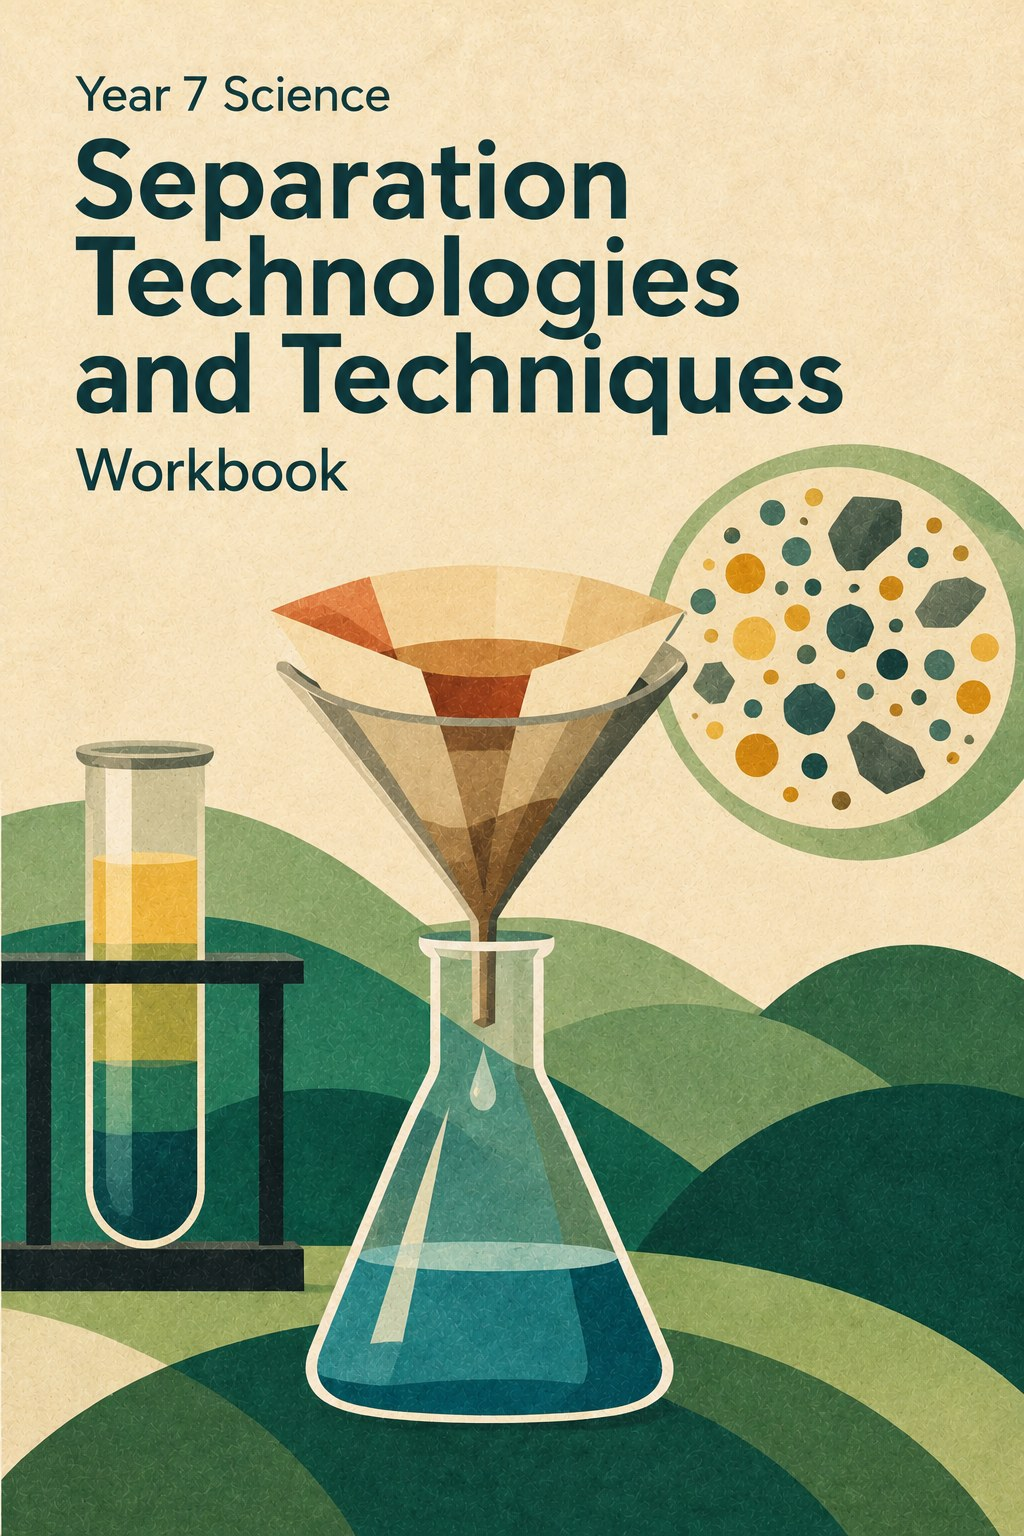
\includegraphics[width=\paperwidth]{../../../covers/separation.jpg}};
  \node[anchor=north east, fill=white, draw=Ink, line width=0.6pt, rounded corners=1.2mm,
        inner xsep=2mm, inner ysep=1.8mm, text width=30mm, font=\headingfont\footnotesize]
    at ([xshift=-4mm, yshift=-4mm]current page.north east)
    {\textbf{Name}\par\vspace{4mm}\hrule\vspace{2mm}\textbf{Class}\par\vspace{4mm}\hrule};
  \node[anchor=south east, fill=white, draw=Ink, line width=0.6pt, rounded corners=1.2mm,
        inner xsep=2.6mm, inner ysep=2mm, font=\headingfont\bfseries, align=right]
    at ([xshift=-4mm, yshift=6mm]current page.south east)
    {Lesson Booklet 2\\[-1pt]{\normalfont\headingfont\scriptsize Lessons 8--16}};
\end{tikzpicture}
\mbox{}
\clearpage

% ---- Inside cover ---------------------------------------------------------
\thispagestyle{plain}
{\headingfont\bfseries\fontsize{16}{20}\selectfont Separation Technologies and Techniques}\par\vspace{1mm}
{\headingfont\large Lesson Booklet 2 \textbullet\ Lessons 8--16 \textbullet\ Year 7}\par\vspace{1mm}
{\small\itshape VC 2.0: VC2S8U05 \textbullet\ VC2S8U06 \textbullet\ VC2S8U07 \textbullet\ VC2S8I01--I08 \textbullet\ VC2S8H02}\par\vspace{4mm}
\textbf{Teacher}\ \hrulefill\par

\begin{countrybox}{Acknowledgement of Country}
This booklet was created on the unceded Country of the Wurundjeri Woi-wurrung people of the Kulin Nation. We acknowledge Elders past, present and emerging.
\end{countrybox}

\begin{infobox}{How this booklet works}
One section for each lesson. Each opens with its key vocabulary, then:\par\smallskip
\renewcommand{\arraystretch}{1.25}
\begin{tabular}{@{}p{24mm}p{70mm}@{}}
\textbf{Part A} & a reading with comprehension questions \\
\textbf{Part B} & the ideas, worked through \\
\textbf{Part C} & practice on your own \\
\textbf{Part D} & above level: Year 8 extension \\
\end{tabular}

\smallskip
\begin{tabular}{@{}p{24mm}p{70mm}@{}}
\textbf{I do} \tagicon{\icodots{1}} & your teacher works an example (solid frame) \\
\textbf{We do} \tagicon{\icodots{2}} & you try one together (dashed frame) \\
\textbf{Reading} \tagicon{\icoread} & a passage to read (thin frame) \\
\textbf{Above level} \tagicon{\icoup} & extension (double frame) \\
\end{tabular}

\smallskip
Two lesson books; experiments are in the \textbf{Experiment Booklet}.
\end{infobox}

\clearpage
\markboth{Contents}{Contents}
{\headingfont\bfseries\LARGE Contents}\par\vspace{1mm}\noindent\rule{\linewidth}{0.6pt}\par\vspace{2mm}
\renewcommand{\arraystretch}{1.45}
\begin{tabular}{|C{1.1cm}|L{6.0cm}|C{2.4cm}|}
  \hline\thead{Lesson} & \thead{Title} & \thead{Page} \\ \hline
  1 & Pure Substances & Book 1 \\ \hline
  2 & Mixtures & Book 1 \\ \hline
  3 & \textit{Experiment 1 --- Solubility} & Experiment Booklet \\ \hline
  4 & Classifying With Particle Diagrams & Book 1 \\ \hline
  5 & Solute, Solvent and Solution & Book 1 \\ \hline
  6 & \textit{Experiment 2 --- Surface Area and Dissolving} & Experiment Booklet \\ \hline
  7 & Decanting, Filtration and Magnetic Separation & Book 1 \\ \hline
  8 & \hyperlink{lesson.8.1}{Evaporation and Crystallisation} & \hyperlink{lesson.8.1}{p.\ \pageref{sec:26}} \\ \hline
  9 & \textit{Experiment 3 --- Fast and Slow Evaporation} & Experiment Booklet \\ \hline
  10 & \hyperlink{lesson.10.1}{Solubility and Saturation} & \hyperlink{lesson.10.1}{p.\ \pageref{sec:20}} \\ \hline
  11 & \textit{Experiment 4 --- Rates of Evaporation} & Experiment Booklet \\ \hline
  12 & \hyperlink{lesson.12.1}{Solubility Curves} & \hyperlink{lesson.12.1}{p.\ \pageref{sec:21}} \\ \hline
  13 & \textit{Experiment 5 --- Solubility and Temperature} & Experiment Booklet \\ \hline
  14 & \textit{Experiment 6 --- Growing Copper Sulfate Crystals (stretch)} & Experiment Booklet \\ \hline
  15 & \textit{Experiment 7 --- Filtration} & Experiment Booklet \\ \hline
  16 & \hyperlink{lesson.16.1}{Distillation and Chromatography} & \hyperlink{lesson.16.1}{p.\ \pageref{sec:27}} \\ \hline
  17 & \textit{Experiment 8 --- Distillation} & Experiment Booklet \\ \hline
  18 & \textit{Experiment 9 --- The Great Green Mix Up} & Experiment Booklet \\ \hline
  --- & \hyperlink{glossary}{Glossary} & \hyperlink{glossary}{\pageref{sec:glossary}} \\ \hline
\end{tabular}
\renewcommand{\arraystretch}{1}
\clearpage
\setcounter{section}{7}\renewcommand{\lessonart}{26}
% ══════════════════════════════════════════════════════════════════════════════
%  LESSON 26 — EVAPORATION AND CRYSTALLISATION                      (Week 9 · P2)
% ══════════════════════════════════════════════════════════════════════════════
\sectiondiv{Evaporation and Crystallisation}{Getting a dissolved solid back \textbullet{} Evaporating to dryness \textbullet{} Growing crystals \textbullet{} Dissolving to separate}\label{sec:26}
\lessoncodes{VC2S8U06 \textbullet{} VC2S8I03}

\vocabhead
\begin{ctab}
\begin{tabular}{|SW{2.91cm}|W{8.05cm}|}
  \hd & \thead{Word} & \thead{Definition (copy from the slide)} \\ \hline
  & \scaf{\textbf{Evaporating to dryness}\label{voc:evaporating-to-dryness}} & \scaf{Heating a solution until all the solvent has gone, leaving the solid behind.} \\ \hline
  & \textbf{Crystallisation}\label{voc:crystallisation} & \\ \hline
  & \textbf{Evaporating basin}\label{voc:evaporating-basin} & \\ \hline
  & \textbf{Leaching}\label{voc:leaching} & \\ \hline
  & \textbf{Salt pan}\label{voc:salt-pan} & \\ \hline
  & \textbf{Impurity}\label{voc:impurity} & \\ \hline
\end{tabular}
\end{ctab}

% ─── PART A ───────────────────────────────────────────────────────────────────
\lessonpart{A}{Reading and comprehension}{Teal}\label{read:26}

\begin{readingbox}{Reading --- Salt From the Sea}
Filtration cannot get salt out of sea water, because the salt is dissolved and passes straight through the paper. To get a dissolved solid back, you have to get rid of the solvent instead. In a laboratory, the solution is heated gently in a shallow \textbf{evaporating basin} until the water has gone and only the solid is left. This is called \textbf{evaporating to dryness}. It is quick, but the crystals it makes are tiny, and anything else that was dissolved is left behind as an \textbf{impurity} too.

Much of the world's salt is made in the same way, but using the Sun. Sea water is let into huge, shallow ponds called \textbf{salt pans}. Over weeks, the Sun and wind evaporate the water, and salt is left behind as a crust that can be scraped up. South Australia and Western Australia both have large salt fields.

If you want big, beautiful crystals, evaporate slowly. This is \textbf{crystallisation}. A saturated solution (one holding as much solute as it can) left in a dish for several days loses its water a little at a time, and the solute particles have time to settle neatly into a regular pattern. The slower the evaporation, the larger and more regular the crystals.

Separation can also work the other way round: instead of removing the water, you use water to remove a dissolved substance. The seeds of some cycad plants are a valuable food but contain a poison. Aboriginal peoples in several parts of Australia made them safe to eat by soaking or washing the prepared seeds in water, often for days or weeks, so that the poison dissolved and was carried away. Removing a soluble substance by washing it out with water is called \textbf{leaching}.
\end{readingbox}

\rcreset
\rcq{Why can filtration not separate salt from sea water?}{1.6cm}
\rcq{Describe how a solid is evaporated to dryness in a laboratory.}{1.8cm}
\rcq{Give two disadvantages of evaporating to dryness.}{1.6cm}
\rcq{How are salt pans used to make salt?}{1.8cm}
\rcq{What is the difference between evaporating to dryness and crystallisation?}{1.8cm}
\rcq{Why does slow evaporation make bigger crystals?}{1.8cm}
\rcq{How were cycad seeds made safe to eat?}{1.8cm}
\rcq{Why is leaching ``separation the other way round''?}{1.6cm}

% ─── PART B ───────────────────────────────────────────────────────────────────
\lessonpart{B}{Theory and examples}{Blue}\label{theory:26}

\subsection{Evaporating to Dryness}\label{sub:26.1}

\diagEvaporation
\figcap{Evaporating a solution. The water leaves as vapour; the dissolved solid stays in the basin.}

\begin{workedex}{Explaining evaporation to dryness}
Explain, using particles, why salt is left behind when salt water is heated in an evaporating basin.

\medskip
Heating gives the water particles enough energy to \textbf{evaporate} and escape as water vapour. The salt has a much higher boiling point, so its particles stay behind. As the water leaves, the salt particles come together and form solid \textbf{crystals}.
\end{workedex}

\begin{wedo}{Explaining evaporation to dryness}
A blue solution of copper sulfate is heated in an evaporating basin. Predict what is left at the end, and explain, using particles.
\answerbox{3.0cm}
\end{wedo}

\subsection{Crystallisation}\label{sub:26.2}

\begin{ctab}
\begin{tabular}{|L{2.67cm}|L{3.93cm}|L{3.93cm}|}
  \thead{} & \thead{Evaporating to dryness} & \thead{Crystallisation} \\ \hline
  Speed & fast (minutes) & slow (days) \\ \hline
  How & heat until no water is left & leave a saturated solution to evaporate slowly \\ \hline
  Crystals & tiny, powdery & large, regular \\ \hline
  Impurities & all left in the solid & mostly stay in the leftover liquid \\ \hline
\end{tabular}
\end{ctab}

\begin{workedex}{Choosing a method}
A jeweller wants large, perfect crystals of a salt to display. Should she evaporate the solution to dryness or crystallise it? Explain.

\medskip
\textbf{Crystallise it.} Slow evaporation gives the particles time to settle into a regular pattern, so the crystals grow \textbf{large and regular}. Fast heating makes only a fine powder.
\end{workedex}

\begin{wedo}{Choosing a method}
A student needs to find, as quickly as possible, how much salt was dissolved in a cup of sea water. Should she evaporate it to dryness or crystallise it? Explain.
\answerbox{2.6cm}
\end{wedo}

\subsection{Dissolving to Separate}\label{sub:26.3}

\begin{workedex}{Getting salt from rock salt}
Rock salt is salt mixed with sand and grit. Describe how to get clean salt from it.

\medskip
\textbf{1. Dissolve:} stir the crushed rock salt into warm water; the salt dissolves, the sand and grit do not.

\textbf{2. Filter:} the sand and grit are the residue; the salt water is the filtrate.

\textbf{3. Evaporate:} heat the filtrate in an evaporating basin, or leave it to crystallise, to get the salt back.
\end{workedex}

\begin{wedo}{Getting sugar from a mixture}
A bag of sugar has been mixed with sawdust. Describe the steps to get clean, dry sugar back, naming each technique.
\answerbox{3.4cm}
\end{wedo}

% ─── PART C ───────────────────────────────────────────────────────────────────
\lessonpart{C}{Practice}{Amber}\label{prac:26}

Work through every task. For each step, name the technique and what it removes.

\needspace{12\baselineskip}
\task Write the best technique for each job: \textbf{filtration}, \textbf{evaporation to dryness}, \textbf{crystallisation} or \textbf{leaching}.

\vspace{4pt}
\begin{ctab}
\begin{tabular}{|SW{6.22cm}|Z{4.74cm}|}
  \hd & \thead{Job} & \thead{Technique} \\ \hline
  & \scaf{Get sand out of muddy water} & \scaf{filtration} \\ \hline
  & Get large crystals of alum for a display & \\ \hline
  & Quickly find the mass of salt in a solution & \\ \hline
  & Wash a soluble poison out of crushed seeds & \\ \hline
\end{tabular}
\end{ctab}

\taskpair{Explain why salt pans are built in hot, dry, windy places.}{2.6cm}
         {Explain why evaporating to dryness leaves impurities in the salt.}{2.6cm}

\needspace{10\baselineskip}
\task Explain, using particles, why crystals grow larger when a solution evaporates slowly.
\answerbox{2.8cm}

\needspace{10\baselineskip}
\task 200\,mL of sea water is evaporated to dryness in a basin with a mass of 85.0\,g. Afterwards, the basin and salt have a mass of 92.0\,g.
\pt{a}What mass of salt was in the sea water?
\workbox{1.8cm}
\pt{b}How much salt would there be in 1\,L (1000\,mL) of the same sea water?
\workbox{1.8cm}

\needspace{10\baselineskip}
\task Some seeds contain a poison that dissolves in water. Explain, using particles, why soaking the crushed seeds in running water for days removes more poison than soaking whole seeds in still water for an hour.
\answerbox{3.0cm}

% ─── PART D ───────────────────────────────────────────────────────────────────
\lessonpart{D}{Above level}{Violet}\label{ext:26}

\begin{yr8box}
These questions go beyond the Year 7 standard. They ask you to plan and evaluate.

\medskip
\begin{keepext}
\needspace{10\baselineskip}
\exttask When a copper sulfate solution is evaporated to dryness with strong heat, the blue solid left behind turns into a white powder. Suggest why crystallisation is a better method for this substance.
\answerbox{3.0cm}
\end{keepext}

\begin{keepext}
\needspace{10\baselineskip}
\exttask Sea water is about 3.5\% salt by mass. What mass of salt is in 2\,kg (2000\,g) of sea water? How much sea water would a salt pan need to evaporate to produce 1\,kg of salt?
\workbox{3.2cm}
\end{keepext}

\begin{keepext}
\needspace{10\baselineskip}
\exttask Plan how to grow the largest possible crystal of salt at home. Describe what you would do, and explain how each step helps the crystal grow large.
\answerbox{3.4cm}
\end{keepext}

\begin{keepext}
\needspace{10\baselineskip}
\exttask Leaching cycad seeds took days and needed a lot of water. Suggest two things that would make leaching faster, and explain each using the particle model of dissolving.
\answerbox{3.0cm}
\end{keepext}

\end{yr8box}
\newpage
\setcounter{section}{9}\renewcommand{\lessonart}{20}
% ══════════════════════════════════════════════════════════════════════════════
%  LESSON 20 — SOLUBILITY AND SATURATION                            (Week 7 · P2)
% ══════════════════════════════════════════════════════════════════════════════
\sectiondiv{Solubility and Saturation}{Saturated solutions \textbullet{} Solubility as a number \textbullet{} Scaling to other volumes \textbullet{} Temperature and solubility}\label{sec:20}
\lessoncodes{VC2S8U06 \textbullet{} VC2S8I04 \textbullet{} VC2S8I05}

\vocabhead
\begin{ctab}
\begin{tabular}{|SW{2.91cm}|W{8.05cm}|}
  \hd & \thead{Word} & \thead{Definition (copy from the slide)} \\ \hline
  & \scaf{\textbf{Saturated}\label{voc:saturated}} & \scaf{A solution that has dissolved as much solute as it can at that temperature.} \\ \hline
  & \textbf{Solubility}\label{voc:solubility} & \\ \hline
  & \textbf{Unsaturated}\label{voc:unsaturated} & \\ \hline
  & \textbf{Concentrated}\label{voc:concentrated} & \\ \hline
  & \textbf{Dilute}\label{voc:dilute} & \\ \hline
  & \textbf{Crystal}\label{voc:crystal} & \\ \hline
\end{tabular}
\end{ctab}

% ─── PART A ───────────────────────────────────────────────────────────────────
\lessonpart{A}{Reading and comprehension}{Teal}\label{read:20}

\begin{readingbox}{Reading --- One Spoonful Too Many}
Add salt to a glass of water one spoonful at a time, stirring after each. The first few spoonfuls disappear easily. But keep going and eventually salt starts to collect at the bottom of the glass, and no amount of stirring will make it dissolve. The water cannot take any more. The solution is \textbf{saturated}: it has dissolved as much solute as it can at that temperature. Before that point, while it could still dissolve more, it was \textbf{unsaturated}.

How much a substance can dissolve is called its \textbf{solubility}. Scientists give it as a number: the mass of solute that will dissolve in 100\,g of water at a certain temperature. (100\,g of water is 100\,mL.) At 20\,\textdegree C, about 36\,g of salt will dissolve in 100\,g of water, but about 200\,g of sugar will --- sugar is far more soluble than salt.

A solution with a lot of solute in it is \textbf{concentrated}; one with only a little is \textbf{dilute}. A saturated solution is as concentrated as it can be at that temperature.

For most solids, solubility goes up as the temperature rises. Hot water dissolves more sugar than cold water. That gives a neat trick: dissolve as much sugar as you can in hot water, then let it cool. The cool water cannot hold it all, so the extra sugar comes back out as a solid, forming \textbf{crystals}. That is how rock candy is made.
\end{readingbox}

\rcreset
\rcq{How can you tell when a solution has become saturated?}{1.6cm}
\rcq{What is the difference between a saturated and an unsaturated solution?}{1.8cm}
\rcq{Use the passage to write a definition of solubility.}{1.6cm}
\rcq{How much salt dissolves in 100\,g of water at 20\,\textdegree C?}{1.2cm}
\rcq{Which is more soluble at 20\,\textdegree C, salt or sugar? Use numbers from the passage.}{1.6cm}
\rcq{What is the difference between a concentrated and a dilute solution?}{1.6cm}
\rcq{How does temperature usually affect the solubility of a solid?}{1.4cm}
\rcq{Explain how rock candy crystals are made.}{1.8cm}

% ─── PART B ───────────────────────────────────────────────────────────────────
\lessonpart{B}{Theory and examples}{Blue}\label{theory:20}

\subsection{Saturated Solutions}\label{sub:20.1}

\begin{workedex}{Is it saturated?}
A student stirs 40\,g of salt into 100\,g of water at 20\,\textdegree C. The solubility of salt at 20\,\textdegree C is 36\,g per 100\,g of water. What does she see, and is the solution saturated?

\medskip
Only 36\,g can dissolve, so $40 - 36 = \mathbf{4\ g}$ is left undissolved at the bottom. The water has dissolved all it can, so the solution \textbf{is saturated}.
\end{workedex}

\begin{wedo}{Is it saturated?}
Copper sulfate has a solubility of 32\,g per 100\,g of water at 20\,\textdegree C. A student dissolves 20\,g in 100\,g of water at 20\,\textdegree C.
\pt{a}Is the solution saturated or unsaturated? Explain.
\answerbox{1.8cm}
\pt{b}How much more copper sulfate could she dissolve?
\workbox{1.6cm}
\end{wedo}

\subsection{Scaling to Other Amounts of Water}\label{sub:20.2}

Solubility is given per 100\,g of water. Half the water dissolves half as much; twice the water dissolves twice as much.

\begin{workedex}{Scaling solubility}
Salt has a solubility of 36\,g per 100\,g of water at 20\,\textdegree C. How much salt can dissolve in 250\,g of water at 20\,\textdegree C?

\medskip
250\,g is $250 \div 100 = 2.5$ times as much water. \quad Salt that dissolves $= 36 \times 2.5 = \mathbf{90\ g}$
\end{workedex}

\begin{wedo}{Scaling solubility}
Sugar has a solubility of 200\,g per 100\,g of water at 20\,\textdegree C. How much sugar can dissolve in 50\,g of water at 20\,\textdegree C?
\workbox{2.6cm}
\end{wedo}

\subsection{Temperature and Solubility}\label{sub:20.3}

\begin{ctab}
\begin{tabular}{|L{2.56cm}|C{1.34cm}|C{1.34cm}|C{1.34cm}|C{1.34cm}|C{1.34cm}|}
  \thead{Temperature (\textdegree C)} & \thead{0} & \thead{20} & \thead{40} & \thead{60} & \thead{80} \\ \hline
  Potassium nitrate (g per 100\,g water) & 13 & 32 & 64 & 110 & 169 \\ \hline
  Salt (g per 100\,g water) & 36 & 36 & 37 & 37 & 38 \\ \hline
\end{tabular}
\end{ctab}

\begin{workedex}{Using a table}
Use the table to describe how temperature affects the solubility of potassium nitrate.

\medskip
As the temperature rises, the solubility of potassium nitrate \textbf{increases a lot}: from 13\,g at 0\,\textdegree C to 169\,g at 80\,\textdegree C, which is about 13 times as much.
\end{workedex}

\begin{wedo}{Using a table}
Salt's solubility is 36\,g at 0\,\textdegree C and 38\,g at 80\,\textdegree C, per 100\,g of water. Describe how temperature affects the solubility of salt, and compare it with potassium nitrate (13\,g at 0\,\textdegree C, 169\,g at 80\,\textdegree C).
\answerbox{3.0cm}
\end{wedo}

% ─── PART C ───────────────────────────────────────────────────────────────────
\lessonpart{C}{Practice}{Amber}\label{prac:20}

Work through every task. Show your working for every calculation.

\needspace{14\baselineskip}
\task Salt has a solubility of 36\,g per 100\,g of water at 20\,\textdegree C. Decide whether each solution at 20\,\textdegree C is saturated or unsaturated.

\vspace{4pt}
\begin{ctab}
\begin{tabular}{|SW{3.18cm}|Z{2.60cm}|Z{4.76cm}|}
  \hd & \thead{Salt added} & \thead{Water} & \thead{Saturated or unsaturated?} \\ \hline
  & \scaf{20\,g} & \scaf{100\,g} & \scaf{unsaturated (36\,g could dissolve)} \\ \hline
  & 50\,g & 100\,g & \\ \hline
  & 10\,g & 50\,g & \\ \hline
  & 20\,g & 50\,g & \\ \hline
\end{tabular}
\end{ctab}

\taskpair{How much salt can dissolve in 200\,g of water at 20\,\textdegree C? (36\,g per 100\,g)}{2.6cm}
         {How much sugar can dissolve in 25\,g of water at 20\,\textdegree C? (200\,g per 100\,g)}{2.6cm}

\needspace{10\baselineskip}
\task 45\,g of salt is stirred into 100\,g of water at 20\,\textdegree C (solubility 36\,g per 100\,g).
\pt{a}How much salt dissolves?
\workbox{1.6cm}
\pt{b}How much is left at the bottom?
\workbox{1.6cm}
\pt{c}Suggest one way to make more of it dissolve.
\answerbox{1.6cm}

\needspace{10\baselineskip}
\task Explain why ``stir it more'' will not help once a solution is saturated.
\answerbox{2.4cm}

\needspace{10\baselineskip}
\task A saturated solution of potassium nitrate is made in 100\,g of water at 60\,\textdegree C, holding 110\,g. It is cooled to 20\,\textdegree C, where the solubility is 32\,g per 100\,g.
\pt{a}What would you see as it cools?
\answerbox{1.8cm}
\pt{b}What mass of crystals forms?
\workbox{1.8cm}

% ─── PART D ───────────────────────────────────────────────────────────────────
\lessonpart{D}{Above level}{Violet}\label{ext:20}

\begin{yr8box}
These questions go beyond the Year 7 standard. They ask you to plan, calculate and explain exceptions.

\medskip
\begin{keepext}
\needspace{10\baselineskip}
\exttask You need to make exactly 300\,g of saturated salt solution at 20\,\textdegree C (solubility 36\,g per 100\,g of water). How much water and how much salt do you need? Hint: start with the mass of solution made from 100\,g of water.
\workbox{3.2cm}
\end{keepext}

\begin{keepext}
\needspace{10\baselineskip}
\exttask Gases are the opposite of most solids: they are \emph{less} soluble in warm water. Use the particle model to suggest why a gas escapes from warm water more easily.
\answerbox{3.0cm}
\end{keepext}

\begin{keepext}
\needspace{10\baselineskip}
\exttask A ``supersaturated'' solution holds more solute than it should at its temperature. If a single small crystal is dropped in, crystals suddenly spread through the whole solution. Suggest why.
\answerbox{3.0cm}
\end{keepext}

\begin{keepext}
\needspace{10\baselineskip}
\exttask Plan a fair test to compare how soluble salt and sugar are at room temperature. Describe what you would measure, and two things you would keep the same.
\answerbox{3.2cm}
\end{keepext}

\end{yr8box}
\newpage
\setcounter{section}{11}\renewcommand{\lessonart}{21}
% ══════════════════════════════════════════════════════════════════════════════
%  LESSON 21 — SOLUBILITY CURVES                                    (Week 7 · P3)
% ══════════════════════════════════════════════════════════════════════════════
\sectiondiv{Solubility Curves}{Reading a solubility curve \textbullet{} Saturated or not? \textbullet{} Crystals on cooling \textbullet{} Drawing a curve from data}\label{sec:21}
\lessoncodes{VC2S8U06 \textbullet{} VC2S8I04 \textbullet{} VC2S8I05}

\vocabhead
\begin{ctab}
\begin{tabular}{|SW{2.91cm}|W{8.05cm}|}
  \hd & \thead{Word} & \thead{Definition (copy from the slide)} \\ \hline
  & \scaf{\textbf{Solubility curve}\label{voc:solubility-curve}} & \scaf{A graph showing how much of a substance dissolves in 100\,g of water at each temperature.} \\ \hline
  & \textbf{Trend}\label{voc:trend} & \\ \hline
  & \textbf{Interpolate}\label{voc:interpolate} & \\ \hline
  & \textbf{Extrapolate}\label{voc:extrapolate} & \\ \hline
  & \textbf{Crystallise}\label{voc:crystallise} & \\ \hline
  & \textbf{Data}\label{voc:data} & \\ \hline
\end{tabular}
\end{ctab}

% ─── PART A ───────────────────────────────────────────────────────────────────
\lessonpart{A}{Reading and comprehension}{Teal}\label{read:21}

\begin{readingbox}{Reading --- A Graph Instead of a Table}
A table of solubility \textbf{data} gives you the solubility at a few temperatures --- perhaps every 20\,\textdegree C. But what if you need to know the solubility at 35\,\textdegree C? Scientists solve this by plotting the data as a \textbf{solubility curve}: a graph with temperature along the bottom and solubility up the side. A smooth line through the points shows the \textbf{trend}, and you can read the solubility at any temperature from the line.

Reading a value between two of the measured points is called \textbf{interpolating}. It is usually reliable, because you are staying inside the range you measured. Reading a value beyond the measured points, by extending the line, is called \textbf{extrapolating}. It is riskier, because the trend might change outside your data.

Solubility curves are useful in industry. Farmers' fertilisers, medicines and table sugar are all purified by letting them \textbf{crystallise}: a hot, saturated solution is cooled, and because the cool water can hold less, the extra solute comes out as crystals. The solubility curve tells the factory exactly how much will crystallise. If a hot solution holds 110\,g of a substance and the curve shows only 32\,g can stay dissolved when it is cool, then $110 - 32 = 78$\,g of crystals will form.

Not every curve is steep. Some substances, like potassium nitrate, become far more soluble as the water warms. Others, like table salt, barely change at all. The shape of the curve tells you which is which at a glance.
\end{readingbox}

\rcreset
\rcq{What goes on each axis of a solubility curve?}{1.4cm}
\rcq{Why is a solubility curve more useful than a table of data?}{1.8cm}
\rcq{What is the difference between interpolating and extrapolating?}{1.8cm}
\rcq{Why is extrapolating riskier than interpolating?}{1.6cm}
\rcq{Give two products the passage says are purified by crystallising.}{1.4cm}
\rcq{Explain why crystals form when a hot, saturated solution cools.}{1.8cm}
\rcq{In the passage's example, how was the mass of crystals worked out?}{1.6cm}
\rcq{How can you tell from the shape of a curve that a substance's solubility hardly changes?}{1.6cm}

% ─── PART B ───────────────────────────────────────────────────────────────────
\lessonpart{B}{Theory and examples}{Blue}\label{theory:21}

\subsection{Reading a Solubility Curve}\label{sub:21.1}

\diagSolubility{1}
\figcap{Solubility curves for potassium nitrate and salt.}

\begin{skillbox}{Reading a value from a curve}
Find the temperature on the bottom axis. Go straight up to the curve. Go straight across to the side axis and read the solubility. Use a ruler for both lines.
\end{skillbox}

\begin{workedex}{Reading the curve}
Use the curve above to find the solubility of potassium nitrate at 50\,\textdegree C.

\medskip
Up from 50\,\textdegree C to the potassium nitrate curve, then across: about \textbf{85\,g per 100\,g of water}.
\end{workedex}

\begin{wedo}{Reading the curve}
Potassium nitrate's solubility rises smoothly from 64\,g at 40\,\textdegree C to 110\,g at 60\,\textdegree C, per 100\,g of water.
\pt{a}Estimate its solubility at 50\,\textdegree C, halfway between.
\answerbox{1.4cm}
\pt{b}At 50\,\textdegree C the solubility is about 85\,g per 100\,g of water. A student dissolves 70\,g of potassium nitrate in 100\,g of water at 50\,\textdegree C. Is the solution saturated? Explain.
\answerbox{1.6cm}
\end{wedo}

\subsection{Crystals on Cooling}\label{sub:21.2}

\begin{workedex}{How much crystallises?}
A saturated solution of potassium nitrate in 100\,g of water at 80\,\textdegree C holds 169\,g. It is cooled to 40\,\textdegree C, where the solubility is 64\,g per 100\,g. What mass of crystals forms?

\medskip
Mass of crystals $=$ mass dissolved when hot $-$ mass that can stay dissolved when cool $= 169 - 64 = \mathbf{105\ g}$
\end{workedex}

\begin{wedo}{How much crystallises?}
A saturated solution of potassium nitrate in 100\,g of water at 60\,\textdegree C holds 110\,g. It is cooled to 20\,\textdegree C, where the solubility is 32\,g per 100\,g. What mass of crystals forms?
\workbox{2.6cm}
\end{wedo}

% ─── PART C ───────────────────────────────────────────────────────────────────
\lessonpart{C}{Practice}{Amber}\label{prac:21}

Work through every task. Use a ruler when you read the graph.

\needspace{30\baselineskip}
\task Use this solubility curve to answer the questions.
\diagSolubility{1}
\pt{a}What is the solubility of potassium nitrate at 30\,\textdegree C?
\answerbox{1.4cm}
\pt{b}At what temperature does 140\,g of potassium nitrate dissolve in 100\,g of water?
\answerbox{1.4cm}
\pt{c}At about what temperature do salt and potassium nitrate have the same solubility?
\answerbox{1.4cm}
\pt{d}Which substance's solubility is affected more by temperature? Explain using the shapes of the curves.
\answerbox{2.2cm}

\needspace{10\baselineskip}
\task 50\,g of potassium nitrate is added to 100\,g of water at 20\,\textdegree C, where its solubility is 32\,g per 100\,g.
\pt{a}Is the solution saturated? How much is undissolved?
\workbox{1.8cm}
\pt{b}The water is warmed to 40\,\textdegree C, where the solubility is 64\,g per 100\,g. What happens to the undissolved solid? Explain.
\answerbox{2.0cm}

\needspace{24\baselineskip}
\task A class measured the solubility of a substance called potassium chloride. Draw a solubility curve of their data on the grid. Use \textbf{temperature (\textdegree C)} on the horizontal axis and \textbf{solubility (g per 100\,g of water)} on the vertical axis.

\vspace{3pt}
\begin{ctab}
\begin{tabular}{|SW{3.39cm}|Z{1.18cm}|Z{1.18cm}|Z{1.18cm}|Z{1.18cm}|Z{1.18cm}|}
  \hd & \thead{Temperature (\textdegree C)} & \thead{0} & \thead{20} & \thead{40} & \thead{60} & \thead{80} \\ \hline
  & Solubility (g per 100\,g) & 28 & 34 & 40 & 46 & 51 \\ \hline
\end{tabular}
\end{ctab}
\graphgrid{11cm}

\needspace{10\baselineskip}
\task The solubility of potassium chloride is 28, 34, 40, 46 and 51\,g per 100\,g of water at 0, 20, 40, 60 and 80\,\textdegree C.
\pt{a}Interpolate the solubility at 30\,\textdegree C.
\answerbox{1.4cm}
\pt{b}Extrapolate the solubility at 100\,\textdegree C, and say how confident you are.
\answerbox{2.0cm}

% ─── PART D ───────────────────────────────────────────────────────────────────
\lessonpart{D}{Above level}{Violet}\label{ext:21}

\begin{yr8box}
These questions go beyond the Year 7 standard. They ask you to scale, combine and evaluate.

\medskip
\begin{keepext}
\needspace{10\baselineskip}
\exttask A saturated solution of potassium nitrate is made in 50\,g of water at 80\,\textdegree C (solubility 169\,g per 100\,g of water) and cooled to 20\,\textdegree C (32\,g per 100\,g). What mass of crystals forms? Show your working.
\workbox{3.2cm}
\end{keepext}

\begin{keepext}
\needspace{10\baselineskip}
\exttask Cooling a salt solution from 80\,\textdegree C to 20\,\textdegree C produces only about 2\,g of crystals per 100\,g of water (38\,g down to 36\,g). Suggest a better way to get salt crystals out of salt water, and explain why it works better.
\answerbox{3.0cm}
\end{keepext}

\begin{keepext}
\needspace{10\baselineskip}
\exttask A mixture contains 60\,g of potassium nitrate and 10\,g of salt, dissolved in 100\,g of water at 80\,\textdegree C. It is cooled to 20\,\textdegree C. At 20\,\textdegree C, 32\,g of potassium nitrate and 36\,g of salt can stay dissolved in 100\,g of water. Which substance crystallises out, and how much? Explain how this could be used to purify potassium nitrate.
\answerbox{3.4cm}
\end{keepext}

\end{yr8box}
\newpage
% Lessons 22-24 are Assessment 1 (separate investigation booklet): keep
% section numbers equal to lesson numbers.
\setcounter{section}{24}
\newpage
\setcounter{section}{15}\renewcommand{\lessonart}{27}
% ══════════════════════════════════════════════════════════════════════════════
%  LESSON 27 — DISTILLATION AND CHROMATOGRAPHY                      (Week 9 · P3)
% ══════════════════════════════════════════════════════════════════════════════
\sectiondiv{Distillation and Chromatography}{Getting the solvent back \textbullet{} How distillation works \textbullet{} Separating dyes \textbullet{} Making drinking water}\label{sec:27}
\lessoncodes{VC2S8U06 \textbullet{} VC2S8I03}

\vocabhead
\begin{ctab}
\begin{tabular}{|SW{2.91cm}|W{8.05cm}|}
  \hd & \thead{Word} & \thead{Definition (copy from the slide)} \\ \hline
  & \scaf{\textbf{Distillation}\label{voc:distillation}} & \scaf{Boiling a liquid and condensing the vapour, to get the liquid back on its own.} \\ \hline
  & \textbf{Condenser}\label{voc:condenser} & \\ \hline
  & \textbf{Distillate}\label{voc:distillate} & \\ \hline
  & \textbf{Chromatography}\label{voc:chromatography} & \\ \hline
  & \textbf{Desalination}\label{voc:desalination} & \\ \hline
  & \textbf{Solvent front}\label{voc:solvent-front} & \\ \hline
\end{tabular}
\end{ctab}

% ─── PART A ───────────────────────────────────────────────────────────────────
\lessonpart{A}{Reading and comprehension}{Teal}\label{read:27}

\begin{readingbox}{Reading --- Water From the Sea, Colours From the Ink}
Evaporating sea water gives you the salt, but the water escapes into the air. What if it is the water you want? Then you use \textbf{distillation}. The salt water is boiled in a flask. Only the water turns into vapour, because salt boils at a far higher temperature. The vapour travels into a \textbf{condenser}, a tube cooled by cold water flowing around it. There it condenses back into pure liquid water, called the \textbf{distillate}, which drips into a beaker. The salt stays behind in the flask.

Turning sea water into fresh water is called \textbf{desalination}. Some desalination plants around the world distil sea water, but distillation uses a lot of energy to boil the water. Australia's big plants, including the one at Wonthaggi in Victoria, push sea water at high pressure through an extremely fine filter instead. Ordinary drinking water from a reservoir is cleaned in other steps: the water is screened, dirt is allowed to settle, it is filtered through beds of sand, and it is disinfected to kill germs.

A different problem is separating several dissolved substances that are mixed together, like the dyes in a black felt-tip pen. For this, scientists use \textbf{chromatography}. A dot of ink is put on a strip of paper just above some water. The water soaks up the paper, and as it passes the ink, it carries the dyes with it. Some dyes travel quickly up the paper; others are held back and travel slowly. Before long, the single dot has spread into separate coloured spots. The highest point the water reaches is called the \textbf{solvent front}. Police scientists use chromatography to tell which pen wrote a forged note.
\end{readingbox}

\rcreset
\rcq{When would you use distillation rather than evaporating to dryness?}{1.6cm}
\rcq{Why does only the water turn into vapour when salt water is boiled?}{1.6cm}
\rcq{What does the condenser do?}{1.6cm}
\rcq{What is the distillate in the passage's example?}{1.2cm}
\rcq{Why do Australia's big desalination plants not use distillation? What do they use?}{1.8cm}
\rcq{List the steps used to clean drinking water from a reservoir.}{1.8cm}
\rcq{Explain how chromatography separates the dyes in black ink.}{2.0cm}
\rcq{How might police scientists use chromatography?}{1.6cm}

% ─── PART B ───────────────────────────────────────────────────────────────────
\lessonpart{B}{Theory and examples}{Blue}\label{theory:27}

\subsection{How Distillation Works}\label{sub:27.1}

\needspace{8cm}
\diagDistillation
\figcap{Simple distillation. The vapour condenses in the cooled condenser and drips into the beaker as distillate.}

\begin{workedex}{Explaining distillation}
Explain, using particles, how distillation gets pure water from salt water.

\medskip
\textbf{In the flask:} heating gives the water particles enough energy to \textbf{boil} and escape as vapour. The salt particles stay behind.

\textbf{In the condenser:} the cold water around the tube takes energy from the vapour. The water particles slow down and \textbf{condense} back into liquid, which drips out as pure distillate.
\end{workedex}

\begin{wedo}{Explaining distillation}
Inky water (water with blue ink dissolved in it) is distilled. Predict the colour of the distillate and what is left in the flask. Explain your answer.
\answerbox{3.0cm}
\end{wedo}

\subsection{Separating Dyes With Chromatography}\label{sub:27.2}

\needspace{7.5cm}
\diagChromatography
\figcap{Paper chromatography. The ink spot starts on a pencil line above the solvent, and separates into its dyes as the solvent rises.}

\begin{skillbox}{Doing chromatography well}
Draw the start line in \textbf{pencil}, not pen --- ink would run. Put the spot \textbf{above} the solvent, or it will dissolve into the beaker. Take the paper out before the solvent reaches the top, and mark the solvent front.
\end{skillbox}

\begin{workedex}{Reading a chromatogram}
A black ink separates into three spots: yellow near the bottom, red in the middle and violet near the top. How many dyes are in the ink, and which travels furthest?

\medskip
Three spots means \textbf{three dyes}. The \textbf{violet} dye travels furthest, so it is carried most easily by the solvent.
\end{workedex}

\begin{wedo}{Reading a chromatogram}
A green felt-tip pen is tested. Its spot separates into a blue spot high up the paper and a yellow spot lower down.
\pt{a}How many dyes are in the green ink?
\answerbox{1.4cm}
\pt{b}Which dye is carried most easily by the solvent? Explain how you know.
\answerbox{1.8cm}
\end{wedo}

\subsection{Choosing the Right Technique}\label{sub:27.3}

\begin{workedex}{Choosing a technique}
You need to collect pure water from muddy, salty water. Which techniques should you use, and in what order?

\medskip
\textbf{1. Filter} to remove the mud, which is insoluble.

\textbf{2. Distil} the filtrate. The water boils off and condenses as pure distillate; the salt stays in the flask.
\end{workedex}

\begin{wedo}{Choosing a technique}
For each job, name the technique you would use: \textbf{(a)} getting pure ethanol out of a mixture of ethanol and water; \textbf{(b)} finding out whether two lollies use the same food colourings.
\pt{a}Ethanol and water.
\answerbox{1.6cm}
\pt{b}Lolly colourings.
\answerbox{1.6cm}
\end{wedo}

% ─── PART C ───────────────────────────────────────────────────────────────────
\lessonpart{C}{Practice}{Amber}\label{prac:27}

Work through every task. Name each technique and the property it uses.

\needspace{14\baselineskip}
\task Complete the table of separation techniques.

\vspace{4pt}
\begin{ctab}
\begin{tabular}{|SW{2.85cm}|W{3.99cm}|W{3.70cm}|}
  \hd & \thead{Technique} & \thead{Property it uses} & \thead{Example} \\ \hline
  & \scaf{Filtration} & \scaf{insoluble solids cannot pass through paper} & \scaf{sand from water} \\ \hline
  & Evaporation & & \\ \hline
  & Distillation & & \\ \hline
  & Chromatography & & \\ \hline
  & Magnetic separation & & \\ \hline
\end{tabular}
\end{ctab}

\taskpair{Why is the start line in chromatography drawn in pencil?}{2.4cm}
         {Why must cold water flow around the condenser?}{2.4cm}

\needspace{10\baselineskip}
\task Explain why distillation gives you the water from salt water, but evaporation to dryness does not.
\answerbox{2.8cm}

\needspace{10\baselineskip}
\task Three pens, A, B and C, were tested with chromatography alongside the ink from a forged note. Pen A gave a blue and a red spot. Pen B gave one black spot. Pen C gave a blue, a red and a yellow spot. The note's ink gave a blue, a red and a yellow spot at the same heights as pen C. Which pen wrote the note? Explain.
\answerbox{2.6cm}

\needspace{10\baselineskip}
\task A town's drinking water comes from a river. Put these treatment steps in a sensible order, and say what each one removes: \emph{disinfect with chlorine}, \emph{filter through sand}, \emph{screen out sticks and leaves}, \emph{let fine dirt settle}.
\answerbox{3.4cm}

% ─── PART D ───────────────────────────────────────────────────────────────────
\lessonpart{D}{Above level}{Violet}\label{ext:27}

\begin{yr8box}
These questions go beyond the Year 7 standard. They ask you to use data from chromatograms and boiling points.

\medskip
\begin{keepext}
\needspace{10\baselineskip}
\exttask Scientists compare spots using the $R_f$ value: the distance the spot moved divided by the distance the solvent front moved. A dye moved 3.0\,cm while the solvent front moved 7.5\,cm. Calculate its $R_f$ value. Why must every $R_f$ value be less than 1?
\workbox{2.6cm}
\end{keepext}

\begin{keepext}
\needspace{10\baselineskip}
\exttask Ethanol boils at 78\,\textdegree C and water at 100\,\textdegree C. A mixture of the two is heated slowly, and the thermometer at the top of the flask is watched. Describe what you would expect the thermometer to show, and explain how this lets you collect mostly ethanol first.
\answerbox{3.4cm}
\end{keepext}

\begin{keepext}
\needspace{10\baselineskip}
\exttask Distillation needs a lot of energy because water must be boiled. Suggest one way a solar still in the desert could make drinking water without fuel. Sketch and label your idea.
\drawbox{5.5cm}{}
\end{keepext}

\end{yr8box}

\clearpage\markboth{Glossary}{Glossary}\hypertarget{glossary}{}\pdfbookmark[1]{Glossary}{glossarybm}
{\headingfont\bfseries\LARGE Glossary}\label{sec:glossary}\par\vspace{1mm}\noindent\rule{\linewidth}{0.6pt}\par
{\small Every key word in this booklet and the page it is introduced on.}\par\smallskip
\renewcommand{\arraystretch}{1.3}
\begin{longtable}{|>{\RaggedRight}p{34mm}|p{9mm}|p{\dimexpr\linewidth-43mm-6\tabcolsep-4\arrayrulewidth-1pt\relax}|}
\hline \rule{0pt}{4mm}\headingfont\bfseries Word & \headingfont\bfseries Page & \headingfont\bfseries In my own words \\ \hline \endhead
  Chromatography & \pageref{voc:chromatography} & \\ \hline
  Concentrated & \pageref{voc:concentrated} & \\ \hline
  Condenser & \pageref{voc:condenser} & \\ \hline
  Crystal & \pageref{voc:crystal} & \\ \hline
  Crystallisation & \pageref{voc:crystallisation} & \\ \hline
  Crystallise & \pageref{voc:crystallise} & \\ \hline
  Data & \pageref{voc:data} & \\ \hline
  Desalination & \pageref{voc:desalination} & \\ \hline
  Dilute & \pageref{voc:dilute} & \\ \hline
  Distillate & \pageref{voc:distillate} & \\ \hline
  Distillation & \pageref{voc:distillation} & \\ \hline
  Evaporating basin & \pageref{voc:evaporating-basin} & \\ \hline
  Evaporating to dryness & \pageref{voc:evaporating-to-dryness} & \\ \hline
  Extrapolate & \pageref{voc:extrapolate} & \\ \hline
  Impurity & \pageref{voc:impurity} & \\ \hline
  Interpolate & \pageref{voc:interpolate} & \\ \hline
  Leaching & \pageref{voc:leaching} & \\ \hline
  Salt pan & \pageref{voc:salt-pan} & \\ \hline
  Saturated & \pageref{voc:saturated} & \\ \hline
  Solubility & \pageref{voc:solubility} & \\ \hline
  Solubility curve & \pageref{voc:solubility-curve} & \\ \hline
  Solvent front & \pageref{voc:solvent-front} & \\ \hline
  Trend & \pageref{voc:trend} & \\ \hline
  Unsaturated & \pageref{voc:unsaturated} & \\ \hline
\end{longtable}
\padtofour
\end{document}
